\section*{Abstract}

The Lattice Boltzmann method (LBM) is a numerical method based on computational statistical mechanics that is well-suited for approximating complex flow behaviors such as non-Newtonian, free surface, and multiphase multicomponent flow.
LBM is typically applied to simulate flow through a series of time steps, each consisting of streaming particle distributions to neighboring nodes and collisions of particle distributions at each node through a collision operator.
The collision operator is of interest because it, along with the equilibrium distribution function, determine the physics that are simulated (e.g. constitutive laws, interfacial dynamics, etc.) and it has implications on numerical stability and computational efficiency.
This work examines various collision operators and methods for stability enhancement for their suitability for simulating non-Newtonian fluid flows in terms of their accuracy, numerical stability and computational efficiency.
The investigation was carried out as a numerical study looking for qualitative, yet practical, results, including testing the BGK and MRT collision operators, with and without entropic filtering, as applied to Bingham plastics and power-law fluids.
Two different benchmark problems were chosen for the flows: Poiseuille flow, and lid-driven square cavity flow.
The results of the numerical study showed that the MRT collision operator can have an advantage in terms of stability and accuracy for a variety of non-Newtonian flow behaviors, but at an increased computing cost that was, in some cases, as much as five times greater than the BGK collision operator.
It was also shown that artificial dissipation can be an effective technique for enhancing the numerical stability of non-Newtonian, lid-driven cavity flow simulations, and is particularly effective for efficiently and accurately simulating the flow of shear-thinning fluids.

\section{Introduction}

There are a number of fluids in science and engineering applications that can be classified as non-Newtonian, such as pastes, slurries, molten plastics, polymer solutions, dyes, varnishes, suspensions, and some biomedical liquids such as blood all behave in a non-Newtonian manner~\cite{bohme1987non}.
Of all of the different non-Newtonian behaviors that exist, there are two models under which much of the behaviors may be idealized: yield stress fluids and power-law fluids.
Yield stress fluids, also known as Bingham plastics, do not flow until a threshold value of stress, referred to as its yield stress, is exceeded.
Yield stress flow has been found to be relevant in many applications, such as the flow of pastes, paints, muds, molten plastics and metals, and in some cases, blood~\cite{wang2011lattice}.

Power-law behavior is also known as \emph{shear-thinning} when the apparent viscosity decreases with increasing strain-rate, or \emph{shear-thickening} when the apparent viscosity increases with increasing strain-rate.
Shear-thinning fluids are also known as \emph{pseudoplastics}, and some examples include tomato concentrate, clay and water mixtures, and molten plastics~\cite{irgens2014rheology}.
Shear-thickening fluids are also known as \emph{dilatants}, and a well-known example is a cornstarch and water mixture.

\label{sec:lbm-for-nnf}

Analytical solutions rarely exist for even the simplest non-Newtonian fluid flows because of the complexity that a nonlinear constitutive relationship entails.
It is generally more practical to approximate the flow of non-Newtonian fluids using numerical methods~\cite{syrakos2014performance,owens2002computational,chai2011multiple}.
The lattice Boltzmann method (LBM) is a numerical method for simulating fluid flow that has the advantage (among others) that computing the strain-rate is second-order accurate in space and local to each node~\cite{kruger2010second}.
This means that although an iterative solution is still required to determine the local strain-rate and apparent viscosity, each iterative solution can be done in parallel, by a separate process, as they are independent of each other.
Because hardware architectures have shifted from single, sequential processing systems to parallel processing systems, the local nature of the stress--strain-rate relationship in LBM gives it a distinct advantage for simulating non-Newtonian flow over some other numerical methods.
For example,~\cite{tang2011bingham,chai2011multiple,fallah2012multiple,chen2014simulations,vikhansky2008lattice,wang2008lattice} developed LBM models for simulating yield stress flow.
The LBM model results agreed well when compared to analytical solutions for Bingham plastic Poiseuille flow and values from literature for lid-driven cavity flow, which shows the feasibility of using LBM models for yield-stress fluids.
Examples of LBM models for power-law fluid flow include~\cite{wang2011lattice,wang2015localized,boyd2006second,chai2011multiple}, and blood flows using the K-L, Casson, and Carreau-Yasuda constitutive relationships~\cite{ashrafizaadeh2009comparison}, which have also been successfully verified with benchmarks.

LBM does, however, have its drawbacks.
LBM can be considered as a type of finite-difference scheme for the continuous Boltzmann equation, and as such, has numerical properties in common with finite-difference schemes.
One such consideration is the potential for numerical inaccuracies and instabilities ~\cite{sterling1993stability,sterling1996stability,bawazeer2013stability,lallemand2000theory}.
%Much work has been done to investigate and develop ways to enhance the stability of lattice Boltzmann methods.
Stability concerns are just as prevalent, if not more prevalent, in simulating non-Newtonian fluids because the nonlinear relationship between shear stress and strain-rate can lead to highly nonlinear fluctuations.
Various strategies for incorporating the physics of non-Newtonian flow with LBM while maintaining a stable numerical method have been developed and studied.
The simplest approach for simulating a shear-rate dependent viscosity is to make the collision frequency, which is proportional to apparent viscosity, variable and dependent on the local strain-rate~\cite{boyd2006second,chen2014simulations,fallah2012multiple,tang2011bingham,svec2011flow,svec2012free,zhao2016lattice}.
A potential issue with the stability of the variable relaxation time approach is that as the collision frequency approaches $2$ the viscosity approaches zero and overrelaxation occurs.
Alternatively, if the relaxation time is much greater than one, the accuracy and stability of the method degrades~\cite{latt2007hydrodynamic}. 
In order to ensure that the variable collision frequencies did not approach values leading to numerical instabilities,~\cite{svec2011flow,svec2012free,gabbanelli2005lattice} set upper and lower bounds on allowable collision frequencies.
Although bounding the collision frequency was shown to be effective in terms of stability, it is nonphysical and can lead to approximations that are inaccurate, not because of round-off error or numerical instability, but because the collision does not reflect the proper constitutive relationship of interest.
Another scheme for incorporating non-Newtonian effects into LBM is to use a constant collision frequency, typically unity, and to instead incorporate the local shear-rate effect through equilibrium distribution functions.
This means particle distribution functions will always relax toward equilibrium at the same rate, but that the definition of equilibrium is modified to represent the correct stress--strain-rate relationship.
The equilibrium distribution function can be derived for a specific constitutive relationship of interest using the Chapman-Enskog multiscale expansion.
The equilibrium distribution functions for Bingham plastic fluids, and for power-law and Carreau fluids were derived, implemented, and verified in~\cite{wang2008lattice} and~\cite{yoshino2007numerical}, respectively.
Using an equilibrium distribution function that incorporates the local strain-rate effect has the advantage that, because the collision frequency is constant (at unity), the collision frequency will not approach values that lead to overrelaxation (e.g. $2$) or underrelaxation (e.g. $\approx 0$).
\cite{wang2011lattice} developed another constant collision frequency LBM scheme for non-Newtonian flow by splitting the effects of constitutive relationship into Newtonian and non-Newtonian parts.
The Newtonian part was modeled in the usual way, namely scaling the collision frequency to achieve the macroscopic (Newtonian) viscosity, and the non-Newtonian part was modeled as a source of momentum (i.e. as an external forcing term) that is dependent on local shear-rate.
Although the constant collision frequency strategies present interesting alternatives, the variable collision frequency scheme is used in the present study because of its simplicity and generality, such as the fact that a variable collision frequency scheme can be fit to any constitutive relationship without performing Chapman-Enskog multiscale expansion.

%The Bhatnagar, Gross, Krook (BGK) collision operator~\cite{bhatnagar1954model}.
The Multiple-relaxation-time (MRT) collision operator ~\cite{d1994generalized} is another approach that has been developed to improve the stability of LBM.
The MRT collision takes place in moment space and allows each moment to relax at a different rate.
\cite{lallemand2000theory} used von Neumann stability analysis to investigate the stability of the newly constructed LBM-MRT model for fluid flow, and concluded LBM with the MRT collision operator was more stable, but with increased computational expense than the commonly used collision operator.
Note that although this increased computational expense was decided to not be significant for Newtonian flow ($\approx$ 10--20\%~\cite{lallemand2000theory}), the cost may increase significantly for non-Newtonian flow if an iterative solution is used for the nonlinear constitutive equation because it can require that certain expensive computations be performed multiple times per time step.
\cite{chen2014simulations} concluded that the MRT collision operator was more stable for Bingham plastic flow and allowed the use of a more accurate approximation to the Bingham plastic constitutive relationship.
However, what remains unclear is:
\begin{itemize}
    \item What is the increased cost associated with the MRT collision operator when applied to non-Newtonian flow?
    \item Under what conditions (e.g. material parameters, physical problem, etc.) for Bingham plastic fluid flow is the MRT collision operator necessary to maintain stability and/or accuracy?
    \item Under what conditions (e.g. material parameters, physical problem, etc.) for power-law fluid flow is the MRT collision operator necessary to maintain stability and/or accuracy?
    \item What are additional strategies for increasing stability and accuracy, and what are their associated computational costs?
\end{itemize}
In regards to the last question, much work has been done recently to enhance stability and accuracy of LBM models beyond the MRT collision operator.
\cite{brownlee2006stabilization,brownlee2007stability,brownlee2008nonequilibrium,packwood2009entropy,gorban2014enhancement} have all developed and tested means for introducing artificial dissipation in order to dampen out high frequency, nonphysical oscillations.
Stability enhancement through artificial dissipation and entropic filtering has shown promise, but to the authors' knowledge has not yet been tested for use in simulating the flow of non-Newtonian fluids.

The goal of the present study is to numerically study the implications on accuracy, stability, and efficiency for some of the different strategies for simulating non-Newtonian flow using LBM. The intention of the study is to aid scientists and engineers in understanding which strategy is best suited to their priorities and applications of interest so as to maximize the advantages LBM has in simulating non-Newtonian flow.
Advantages, such as LBM's potential to scale well in parallel, can be much less realized if the collision operator is too computationally expensive, or if numerical instabilities ensue.
A numerical study can help to determine approximate numerical values, domains, and boundary conditions in which one LBM scheme may be more advantageous than another so that LBM may be used in a computationally efficient and stable manner.
In \Fref{sec:LBM}, an overview of the Lattice Boltzmann Method for simulating fluid flow is presented, along with the collision operators, stability enhancements, and constitutive relationships that were investigated.
\Fref{sec:numerical-study} outlines the boundary conditions, material parameters, and LBM collision schemes for each simulation in the numerical study, and is followed by results and discussion.
Finally, concluding remarks are given in \Fref{sec:numerical-study-conclusions}.

\section{Lattice Boltzmann Method for Simulation of Non-Newtonian Fluids} \label{sec:LBM}

The Lattice Boltzmann method is a numerical approach that uses statistical mechanics to represent a variety of physical processes, such as fluid flow.
More specifically, LBM can be thought of as a special finite difference discretization of the Boltzmann equation~\cite{chen1998lattice}.
The length scale of LBM is unique in contrast to most common numerical methods and is referred to as the mesoscale.
In contrast to continuum based methods, LBM simulates the kinetics of microscopic particles, and so it reaches a finer length scale than the macroscopic domain of continuum mechanics; and in contrast to molecular dynamics, discrete element method, and other particle scale approaches, LBM does not deal with a complete description of the degrees of freedom for each individual particle.
LBM instead relies on a statistical description of particle distributions, making LBM, in general, more computationally efficient and requiring less memory than other particle methods.
Thus, LBM can be seen as a compromise between continuum and particle methods, combining strengths from each.

As noted previously, LBM has some advantages over other methods of CFD.
For example, LBM is a computationally efficient approach for some CFD.
This efficiency is a consequence of two distinct features of LBM: (1) the convective operator is linear, as opposed to the nonlinear convection terms that appear in continuum mechanics approaches; and (2) the fluid pressure is given by an equation of state.
Solving for the fluid pressure in traditional method is more computationally expensive and requires special treatment such as iteration and/or relaxation~\cite{chen1998lattice}.

\subsection{The Boltzmann Equation}
The Boltzmann equation (BE) can be thought of as a conservation of particle distributions.
The BE is given as:
\begin{equation}
\frac{\partial f}{\partial t} + \pvel \cdot \grad f = \colop,
\end{equation}
\noindent where $f = f(\pos, \pvel, t)$ is the particle velocity distribution function, $\pos$ is the spatial position vector, $\pvel$ is the particle velocity, and $\colop = \colop(f)$ is the collision operator.
The lattice part of LBM refers to the way in which the BE is discretized.
The lattice discretizes the spatial domain with nodes that are connected to their neighbors through discrete lattice velocity vectors.
The velocity vectors act as pathways for particle distributions to travel along.
Each time step in LBM consists of two distinct actions:

\begin{itemize}
\item Streaming: particle distributions propagate to their neighbors along the lattice velocity vectors.
The particles can only move along the vectors in their specified direction and can only move at a specific speed.
\item Collision: particle distributions meet at a node and ``collide''.
In LBM, collisions are not simulated in a realistic sense, meaning that each individual particle does not exist and glance off of or interact with one another.
Instead, the collision operator is formulated in such a way that particle distributions are relaxed toward equilibrium.
What defines equilibrium depends on the mechanics of interest to be modeled.
\end{itemize}

The D2Q9 lattice was used in the current work (shown in \Fref{fig:d2q9}), which is commonly used for two-dimensional, incompressible flow simulations~\cite{Suc01}.
The lattice is two-dimensional with nine discrete velocities at each node.
There is a stationary particle, there are four discrete velocities of magnitude 1, $\begin{Bmatrix}1 & 0\end{Bmatrix}^T$, $\begin{Bmatrix}0 & 1\end{Bmatrix}^T$, $\begin{Bmatrix}-1 & 0\end{Bmatrix}^T$, $\begin{Bmatrix}0 & -1\end{Bmatrix}^T$, and there are four discrete velocities of magnitude $\sqrt{2}$, $\begin{Bmatrix}1 & 1\end{Bmatrix}^T$, $\begin{Bmatrix}-1 & 1\end{Bmatrix}^T$, $\begin{Bmatrix}-1 & -1\end{Bmatrix}^T$, $\begin{Bmatrix}1 & -1\end{Bmatrix}^T$.
The discretized version of the Boltzmann equation, or the lattice Boltzmann equation (LBE), is given as:
\begin{equation}
f_i(\pos + \pvel_i \Delta t, t + \Delta t) = f_i(\pos, t) + \colop_i(\pos, t),
\end{equation}
\noindent where, for D2Q9, $i = 0, 1, ..., 8$ is the index of the discrete velocity vector.
\begin{figure}
  \centering
  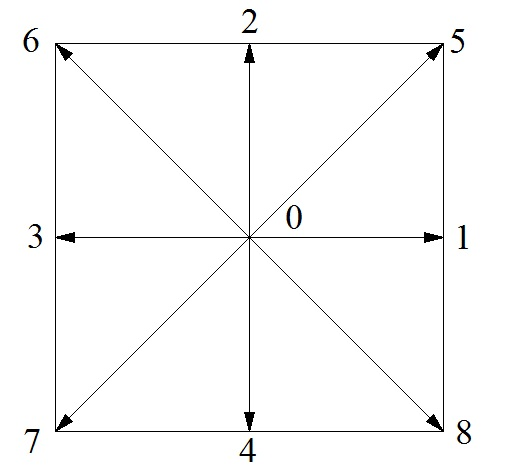
\includegraphics[width=10cm]{figs/d2q9}
  \caption{Schematic of D2Q9 lattice, each node is connected to its neighbor by one of eight discrete velocity vectors}
  \label{fig:d2q9}
\end{figure}

The macroscopic variables of interest can be calculated from the particle distribution functions, $f(\pos, \pvel, t)$, by integrating moments of $f$ over velocity space.
Due to the discrete nature of velocity in LBM, the integrals simply become summations.
The mass density is given by the sum of the particle distributions and the momentum density is given by the first moment of the particle distributions over the velocity space:

\begin{align}
\label{eq:rho} \rho(\pos, t) =& \sum_{i} f_i(\pos, t), \\
\label{eq:mom} \mmom(\pos, t) = \rho(\pos, t) \mvel(\pos, t) =& \sum_{i} \pvel_i f_i(\pos, t)
\end{align}

\noindent The fluid pressure is related to macroscopic density through an equation of state:

\begin{equation}
\label{eq:pres} p(\pos, t) = \rho(\pos, t) c_s^2,
\end{equation}

\noindent where $c_s$ is the lattice speed of sound ($c_s = \frac{1}{\sqrt{3}}$, for D2Q9).

\subsection{Collision Operator} \label{sec:colop}

\subsubsection{Bhatnagar-Gross-Krook} \label{sec:bgk}

The collision operator, in the case of the continuous BE, attempts to describe the change in particle momentums and trajectories due to pairwise particle collisions (based on their respective momentums and trajectories just prior to collision)~\cite{Cer90}.
In LBM, the collision operator causes particle distributions to relax toward a quasiequilibrium. 
This equilibrium is determined by the macroscopic physical behavior of interest (e.g. diffusion, incompressible flow, compressible flow, etc.).
In the case of incompressible flow, the quasiequilibrium particle distribution, $f_i^{eq} = f_i^{eq}(\pos, t)$, is often given by:

\begin{equation} \label{eq:feq}
  f_i^{eq} = w_i \rho \left[1 + \frac{\pvel_i \cdot \mvel}{c_s^2} + \frac{(\pvel_i \cdot \mvel)^2}{4c_s^2} - \frac{\mvel^2}{2c_s^2} \right],
\end{equation}

\noindent where $\rho$ and $\mvel$ are dependent on $\pos$ and $t$, and $w_i$ is the weight in the $i$th:%MG: maybe say something about where this comes from, e.g. feq is a Hermite polynomial expansion of the Maxwell-Boltzmann distribution

\begin{equation} \label{eq:weights}
w_i = \begin{cases}
    \frac{4}{9}, & i = 0 \\
    \frac{1}{9}, & i = 1, 2, 3, 4 \\
    \frac{1}{36}, & i = 5, 6, 7, 8
\end{cases}.
\end{equation}

Due to its simplicity and computational efficiency, the most common collision operator is the Bhatnagar--Gross--Krook (BGK) operator.
BGK consists of a single relaxation time and is a linear relaxation of particle distributions toward equilibrium.
The BGK collision operator for the $i^{th}$ discrete velocity is expressed as:

\begin{equation} \label{eq:bgk}
\Omega_i(\pos, t) = -\omega (f_i(\pos, t) - f_i^{eq}(\pos, t)),
\end{equation}

\noindent where $\omega$ is the collision frequency~\cite{Bha54}.
The collision frequency can be related to macroscopic constitutive properties through Chapman-Enskog multiscale analysis~\cite{wolf2000lattice}.
For incompressible Newtonian flow, the collision frequency is related to the kinematic viscosity by $\nu = c_s^2(\frac{1}{\omega} - \frac{1}{2})$; and from this relationship it is clear that $\omega \in \begin{bmatrix}0.0,& 2.0\end{bmatrix}$, otherwise the viscosity would be negative.
The method for simulating non-Newtonian flow in the current work involves approximating a solution to the local value of apparent viscosity, $\mu_{app}(\pos, t)$, where the shear stress, $\tau$, and strain-rate, $\dot{\gamma}$, are dependent on $\pos$ and $t$, and then setting the value of the local collision frequency as follows:
\begin{equation} \label{eq:colfreq-non-newtonian}
\omega(\pos, t) = \frac{1}{\frac{\mu_{app}(\pos, t)}{c_s^2 \rho(\pos, t)} + \frac{1}{2}}
\end{equation}

Despite the utility of the BGK collision operator, it does have a few drawbacks.
For example, in low viscosity fluids, the BGK operator results in an overrelaxation of particle distributions toward quasiequilibrium.
It is well known that when large nonequilibrium distributions exist in the LBM approximation that overrelaxation can result in nonphysical oscillations that are slow to decay~\cite{brownlee2007stability,dellar2003incompressible}.
To illustrate this, consider a flow in which there is a sharp spatial gradient in either $\rho$ or $\mvel$ at $\pos$.
As $f_i^{eq}$ depends on both $\rho$ and $\mvel$ \eqref{eq:feq}, it may be the case that $|f_i^{eq}(\pos, t) - f_i^{eq}(\pos + \pvel_i \Delta t, t + \Delta t)| >> 0$, i.e. there may be a large difference in the quasiequilibrium for the $i^{th}$ discrete velocity at $(\pos, t)$ and $(\pos + \pvel_i \Delta t, t + \Delta t)$.
In this case, if $f_i$ is ``near'' to quasiequilibrium at $\pos$ it will be ``far'' from quasiequilibrium after the streaming step when it moves to the node at $\pos + \pvel_i \Delta t$.
Overrelaxation will occur if $\nu \rightarrow 0$ because consequently $\omega \rightarrow 2$ and \eqref{eq:bgk} results in $f_i(\pos + \pvel_i \Delta t,t + \Delta t)$ still being ``far'' from $f^{eq}_i(\pos + \pvel_i \Delta t,t + \Delta t)$ but on the ``other side''.
Overrelaxation in subsequent time steps (along the streaming trajectory of $f_i$) could result in nonphysical oscillations.
Considering the effect oscillations of particle distributions will have on macroscopic variables and, consequently, local quasiequilibriums, positive feedback loops can occur causing the system to diverge or ``pollute'' the system enough to make the results highly nonphysical~\cite{gorban2014enhancement}.

The challenge associated with high viscosity fluids is that particular distributions may never relax as ``far'' toward quasiequilibrium as is physical because $\omega \rightarrow 0$ as $\nu \rightarrow \infty$, resulting in extreme underrelaxation to the point of being negligible.
Concerns with sharp gradients, overrelaxation, and underrelaxation are particularly relevant in non-Newtonian flow because of the nonlinear constitutive relationship between shear stress and strain-rate.
The nonlinear constitutive relationship can lead to sharp gradients in $\rho$ or $\mvel$, and depending on the form of the function $\mu_{app}(\dot{\gamma})$, the local collision frequency may result in overrelaxation in certain parts of the domain and extreme underrelaxation in others.

Due to the instabilities associated with the collision frequency being too high (e.g. approaching 2) or too low (e.g. approaching 0), a natural, albeit nonphysical, approach to using the BGK collision operator for non-Newtonian flow is to simply put bounds on the values in which the collision frequency may attain (such as in~\citet{svec2011flow,svec2012free,gabbanelli2005lattice}).
This simple methodology for increasing stability will henceforth be referred to bounded-relaxation time BGK, or BGK-BRT.

\subsubsection{Multiple-relaxation Time} \label{sec:mrt}

An alternative to the BGK collision operator is the multiple-relaxation-time (MRT) collision operator.
In the LB-MRT scheme, one constructs a space based on the particle velocity, $\pvel$, moments of $\mathbf{f} = \begin{Bmatrix}f_0 & f_1 & ... & f_8\end{Bmatrix}^T$, herein referred to as the ``moment space''.
The collision is then performed in the moment space.
There are a few reasons why it is advantageous to perform the collision in the moment space as opposed to the particle distribution space:
\begin{enumerate}
    \item Physical processes in fluids can be approximately described by coupling or interacting among modes, and the modes are directly related to the moments~\cite{lallemand2000theory}.
    \item For the D2Q9 lattice, there are nine distribution functions, $f_0, f_1, ..., f_8$, but only six variables that affect the intended hydrodynamics on a macroscopic scale, namely: $\rho$, $\mathbf{u}$, and $\mathbf{\Pi}$, where $\mathbf{\Pi}$ is the momentum flux tensor~\cite{dellar2003incompressible}.
    Of the nine relaxation rates available, the three that correspond to the extra variables--often referred to as ``ghost variables'', and their associated modes as ``ghost modes''--can be tuned in order to dampen out their associated ghost modes, ensuring these modes do not dominate or cause numerical instabilities at the lattice scale.
\end{enumerate}

The MRT collision operator is given by:

\begin{equation} \label{eq:mrt-colop}
	\colop = - {\transM}^{-1} \relaxM \transM (\mathbf{f} - \mathbf{f}^{eq}),
\end{equation}

\noindent where $\transM$ is a transformation matrix that maps the particle distribution vector, $\mathbf{f}$, and quasiequilibrium distribution vector, $\mathbf{f}^{eq}$, from the particle distribution space into moment space.
The result of mapping the vectors $\mathbf{f}$ and $\mathbf{f}^{eq}$ into moment space will be denoted by $\mathbf{m}$ and $\mathbf{m}^{eq}$, respectively.
The relationships between $\mathbf{m}$, $\transM$ and $\mathbf{f}$ can be written as follows:

\begin{equation} \label{eq:transformation-matrix}
\mathbf{m} = \begin{bmatrix}
\rho \\ e \\ \epsilon \\ j_x \\ q_x \\ j_y \\ q_y \\ p_{xx} \\ p_{xy}
\end{bmatrix} = \begin{bmatrix}
1 & 1 & 1 & 1 & 1 & 1 & 1 & 1 & 1 \\
-4 & -1 & -1 & -1 & -1 & 2 & 2 & 2 & 2 \\
4 & -2 & -2 & -2 & -2 & 1 & 1 & 1 & 1 \\
0 & 1 & 0 & -1 & 0 & 1 & -1 & -1 & 1 \\
0 & -2 & 0 & 2 & 0 & 1 & -1 & -1 & 1 \\
0 & 0 & 1 & 0 & -1 & 1 & 1 & -1 & -1 \\
0 & 0 & -2 & 0 & 2 & 1 & 1 & -1 & -1 \\
0 & 1 & -1 & 1 & -1 & 0 & 0 & 0 & 0 \\
0 & 0 & 0 & 0 & 0 & 1 & -1 & 1 & -1
\end{bmatrix} \begin{bmatrix}
f_0 \\
f_1 \\
f_2 \\
f_3 \\
f_4 \\
f_5 \\
f_6 \\
f_7 \\
f_8
\end{bmatrix} = \transM \mathbf{f}.
\end{equation}

\noindent where $\epsilon$ is related to the square of the energy $e$; $q_x$ and $q_y$ correspond to the energy fluxes in the x and y directions; and $p_{xx}$ and $p_{xy}$ correspond to the diagonal and off-diagonal component of the viscous stress tensor~\cite{lallemand2000theory}.
The relaxation matrix, $\relaxM$, is a diagonal matrix where each of the elements on the diagonal, $s_i \in [0, 2], i = 0, 1, ..., 8$, correspond to the relaxation rate of its associated hydrodynamic mode.
In the case when $s_0 = s_1 = ... = s_8 = \omega$, the MRT collision operator is equivalent to the BGK collision operator ($\omega$ is the collision frequency in the BGK sense).
The relaxation parameters $s_0$, $s_3$, and $s_5$ are all set to zero as mass and momentum should be conserved.
The relaxation parameters $s_1$ and $s_7 = s_8$ are related to the bulk and shear viscosities, respectively.
The relationship for the shear viscosity is given by:
\begin{equation} \label{eq:mrt-s7}
\nu = c_s^2 \Delta t (\frac{1}{s_7} - \frac{1}{2}),
\end{equation}
\noindent which is equivalent with the relationship to the collision frequency, $\omega$, in the BGK sense (when $\Delta t = 1$).
The remaining relaxation parameters, $s_2$, $s_4$, and $s_6$, are tuned in order to dampen out and separate the ghost modes from the modes affecting hydrodynamic transport.
It is common practice, and~\citet{lallemand2000theory} recommends, that these three relaxation parameters be set to slightly larger than one.

The MRT collision operator has a greater numerical stability than its BGK counterpart~\cite{lallemand2000theory,dellar2003incompressible,d2002multiple}, and because of the challenges associated with simulating non-Newtonian flow, the MRT collision operator has become popular for simulating non-Newtonian fluids~\cite{chen2014simulations,fallah2012multiple,tang2011bingham,vikhansky2008lattice,chai2011multiple,grasinger2015simulation}.
The main drawback of the MRT collision operator is its computational expense.
Why MRT is more computationally expensive is clear when one considers that \eqref{eq:mrt-colop} requires multiple matrix multiplications and \eqref{eq:bgk} requires none.
It has been reported that MRT is approximately 15\% slower than BGK~\cite{d2002multiple}, but this was in the context of Newtonian flow.
As will be shown later, for certain LBM implementations and non-Newtonian fluid flows the increase in computational expense can be much greater.

\subsection{Stability Enhancement through Artificial Dissipation: Entropic Filtering}

To reduce nonequilibrium fluctuations in LBM, one can introduce artificial dissipation.
The idea of artificial dissipation is to increase numerical stability while sacrificing some physical accuracy.
A model that has more physical justification but produces unstable and nonsensical results is much less useful than a model with some minor artificial features yet produces more stable results.
%Lyapanov stability is the idea that solutions at equilibrium stay there.
A practical goal then would be to use only the necessary amount of artificial dissipation in order to ensure a stable solution.
From this goal two questions naturally arise: ``under what criteria does one decide that artificial dissipation is necessary?'' and ``how much artificial dissipation does one introduce when it is necessary?''.

%To answer the first question, consider the discussion in \Fref{sec:bgk} on problems with overrelaxation and nonphysical oscillations.
Nonphysical oscillations due to overrelaxation would be damped out more quickly if particle distributions ``far'' from quasiequilibrium were brought closer to quasiequilibrium.
Thus, a particle distribution vector, $\mathbf{f}$, ``far'' from quasiequilibrium would be a good candidate for artificial dissipation.
However, there are many ways one can measure the distance between $\mathbf{f}$ and $\mathbf{f}^{eq}$; for example, a reasonable choice would be $||\mathbf{f} - \mathbf{f}^{eq}||_p$ for some $p$ norm.
A metric that has been developed and used successfully for determining when artificial dissipation should be introduced at a lattice site is the so-called relative nonequilibrium entropy~\cite{gorban2014enhancement,brownlee2006stabilization,brownlee2007stability,brownlee2008nonequilibrium,packwood2009entropy}.
The relative nonequilibrium entropy, $\Delta S$, is given by:

\begin{equation} \label{eq:rel-noneq-entropy}
\Delta S = \sum_i f_i \ln(\frac{f_i}{f^{eq}_i}).
\end{equation}

\noindent A more computationally efficient approximation of $\Delta S$ can be achieved by instead using the second-order Taylor expansion of \eqref{eq:rel-noneq-entropy}:

\begin{equation} \label{eq:quadratic-entropy}
\Delta S \approx \sum_i \frac{(f_i - f^{eq}_i)^2}{2f^{eq}_i}.
\end{equation}

\noindent Note that limiting nonequilibrium entropy in LBM is analogous to what flux limiters do in finite difference, finite volume, and finite element methods~\cite{brownlee2008nonequilibrium}.

A criteria for introducing artificial dissipation that has been used successfully ~\cite{gorban2014enhancement,brownlee2006stabilization,brownlee2007stability,brownlee2008nonequilibrium} is to define a threshold, $\theta$, such that dissipation is added when:
\begin{equation} \label{eq:ds-threshold}
  \Delta S(\pos, t) > \theta.
\end{equation}
A potential drawback of defining a threshold \textit{a priori} is that in order to ensure the model still retains some physical integrity, only a small number of sites can have artificial dissipation added.
If the threshold is too low, too many sites may have dissipation added.
If the threshold is too high, a stable solution may not be achieved.
The threshold can be determined on a case-by-case basis through trial-and-error or by a preliminary analysis.
In the current work, the criteria that is used for determining whether dissipation should be added is a combination of \eqref{eq:ds-threshold} and the following:

\begin{equation} \label{eq:dissipation-criteria}
  \Delta S(\pos, t) > \overline{\Delta S} + n_\sigma \cdot \sigma_{\Delta S},
\end{equation}

\noindent where $\overline{\Delta S}$ and $\sigma_{\Delta S}$ are the mean and standard deviation of $\Delta S$, respectively--both are calculated using values over the domain for the current time step--and $n_\sigma$ is the number of standard deviations greater than $\overline{\Delta S}$ that $\Delta S$ must be before dissipation is added.
The number of standard deviations, $n_\sigma$, is chosen \textit{a priori}.
The criteria described in \eqref{eq:dissipation-criteria} has the advantage that one does not need to determine \textit{a priori} what constitutes ``far'' from quasiequilibrium, but instead considers the maximum percentage of sites one would want artificial dissipation to be added to.
A disadvantage of \eqref{eq:dissipation-criteria} is that if $\overline{\Delta S}$ and $n_\sigma$ are both small then it is possible for dissipation to be added when $\Delta S(\pos, t)$ is low and artificial dissipation is unnecessary.
By requiring that both \eqref{eq:ds-threshold} and \eqref{eq:dissipation-criteria} be met before artificial dissipation is added, there is the potential for \eqref{eq:ds-threshold} and \eqref{eq:dissipation-criteria} to compensate for the each other's disadvantage.

Just as there are many ways to measure a lattice site's distance from quasiequilibrium and define criteria for artificial dissipation, there are also many different ways of deciding how much dissipation to add.
One method of adding dissipation is the so-called Ehrenfests' regularization~\cite{brownlee2006stabilization} and involves setting a lattice site that is chosen for artificial dissipation to its quasiequilibrium state.
Although this achieves the desired result, namely dampening out large nonequilibrium fluctuations, it does so in a way that is not smooth or gradual, but sharp.
An alternative, the median filter, has been used successfully in conjunction with both the BGK and MRT collision schemes for simulating one-dimensional shock tubes and lid-driven cavity flow~\cite{brownlee2008nonequilibrium,gorban2014enhancement,packwood2009entropy}.
In LBM this is a desirable way to introduce dissipation because it has the potential to reduce high-frequency nonequilibrium fluctuations that might lead to numerical instability while retaining the lower frequency dynamics.
To use the median filter one performs the collision step and then checks over the domain for lattice sites with $\Delta S$ that meet the criteria for artificial dissipation.
Sites that meet the criteria are updated as follows:
\begin{equation} \label{eq:median-filter}
\mathbf{f} = \mathbf{f}^{eq} + \delta (\mathbf{f} - \mathbf{f}^{eq}),
\end{equation}
\noindent where $\delta = \sqrt{\Delta S_{med} / \Delta S}$ is the scaling coefficient, and $\Delta S_{med}$ is the median value of $\Delta S$ for the nearest neighbors of the lattice site.

\subsection{Boundary Conditions and Applied Forces} \label{sec:bcs}

No slip, or zero velocity, which is commonly imposed at walls in a domain, is accomplished by simulating the particle distributions as "bouncing back" at the walls in the opposite direction from which they stream.
For example, for a particle distribution streaming in the direction of a south wall, $f_2 = f_4$, $f_5 = f_7$, and $f_6 = f_8$.
For velocity or pressure boundary conditions, the method proposed by~\citet{zou1997pressure} can be used.
The particle distributions that are missing after the streaming step are solved for by assuming a bounce back of the nonequilibrium distribution in the direction normal to the boundary; e.g., for a south inlet or outlet, $f_2 - f_2^{eq} = f_4 - f_4^{eq}$.

Incorporating external forces, such as gravity, pressure gradients, etc., is done by adding a source of particle distributions in the direction of the force.
The increase in particle distributions leads to the desired macroscopic result, which is an increase in momentum.
The LBE with external forces is:

\begin{equation}
f_i(\pos + \pvel_i \Delta t, t + \Delta t) = f_i(\pos, t) + \Omega_i(f) + \frac{w_i \Delta t}{c_s^2} \mathbf{F} \cdot \pvel_i
\end{equation}

\noindent where $\mathbf{F}$ is the body force vector.

\subsection{Strain-rate Tensor}

In the present work, material behavior is simulated through the collision frequency, $\omega$, when using the BGK collision operator (\Fref{sec:bgk}), or the $s_7$ and $s_8$ relaxation rates when using the MRT collision operator (\Fref{sec:mrt}).
Both the collision frequency and the $s_7$ and $s_8$ relaxation rates are dependent on the apparent viscosity, $\mu_{app}$, through \eqref{eq:colfreq-non-newtonian} and \eqref{eq:mrt-s7}, respectively.
The apparent viscosity, in the context of non-Newtonian flow, is a function of the local strain-rate, $\dot{\gamma}$.
The strain-rate is given by the second invariant of the strain-rate tensor, $\srtensor$, i.e.:
\begin{equation} \label{eq:second-invariant}
\dot{\gamma} = \sqrt{2 \sum_{\alpha,\beta=1}^{2} \srtensor \srtensor}.
\end{equation}

\noindent When using the BGK collision scheme, the strain-rate tensor is determined by:
\begin{equation} \label{eq:srtensor-bgk}
D_{\alpha \beta} = -\frac{\omega}{2 \rho c_s^2} \sum_i \xi_{i \alpha} \xi_{i \beta} (f_i - f^{eq}_i),
\end{equation}

\noindent and for the MRT collision scheme, the strain-rate tensor is determined by:
\begin{equation} \label{eq:srtensor-mrt}
D_{\alpha \beta} = -\frac{1}{2 \rho c_s^2 \Delta t} \sum_i \xi_{i \alpha} \xi_{i \beta} \sum_j (\transM^{-1} \relaxM \transM)_{ij}(f_i - f^{eq}_i).
\end{equation}

\noindent Computing the strain-rate tensor by either \eqref{eq:srtensor-bgk} or \eqref{eq:srtensor-mrt} is second order accurate in space~\cite{kruger2009shear,kruger2010second}.

It can be seen from \eqref{eq:srtensor-bgk} and \eqref{eq:srtensor-mrt} that the strain-rate tensor is a function of the collision frequency in the case of the BGK collision operator, or the relaxation matrix, $\relaxM$, in the case of the MRT collision operator.
This interdependence between the relaxation parameters ($\omega$, $s_7$ and $s_8$) and the strain-rate is a direct result of a nonlinear, non-Newtonian constitutive relationship.
The present work uses a Picard-type algorithm to approximate a solution for $\dot{\gamma}$ and $\mu_{app}$:

\label{sec:picard}
\begin{enumerate}
  \item Start with initial guess for the apparent viscosity, $\mu_{app}^k = \mu_{app}^0$.
	      Set $\omega^k$ using \eqref{eq:colfreq-non-newtonian} (or set $s_7^k = s_8^k$ using \eqref{eq:mrt-s7})
	\item \label{step:solve-for-flow} Solve for the strain-rate, $\dot{\gamma}^k$, using \eqref{eq:srtensor-bgk} (or using \eqref{eq:srtensor-mrt}).
  \item Update the apparent viscosity, $\mu_{app}^{k+1} = \mu_{app}(\dot{\gamma}^k)$.
	\item Return to Step \ref{step:solve-for-flow} until the apparent viscosity estimate converges.
\end{enumerate}
\noindent where $\mu_{app}(\dot{\gamma}^k)$ is form of the constitutive relationship that maps the local strain-rate to a local apparent visocisty.
More detail on the functions that are used for $\mu_{app}(\dot{\gamma}^k)$ is given in \Fref{sec:constit}.

It is clear that calculating the strain-rate tensor for the MRT collision operator is more computationally expensive than it is for the BGK collision operator.
The increase in the overall computational expense for simulating non-Newtonian flow using the MRT collision operator is exacerbated by the fact that approximating the apparent viscosity requires iteration and therefore multiple calculations of the strain-rate tensor for each discrete moment in time and for each discrete location in the domain.

\subsection{Non-Newtonian Constitutive Equations} \label{sec:constit}

\subsubsection{Bingham Plastic} \label{sec:bp}

A Bingham plastic does not flow (i.e. the strain-rate is zero) when the shear stress is below the yield stress and behaves in an almost Newtonian manner when the shear stress is above the yield stress.
The Bingham plastic relationship is described mathematically as:
\begin{equation} \label{eq:bingham}
\begin{cases}
\tau = \tau_y + \mu_p \dot{\gamma}, & |\tau| \geq \tau_y \\
\dot{\gamma} = 0, & |\tau| < \tau_y
\end{cases}
\end{equation}
\noindent where $\tau$ is the shear stress, $\tau_y$ is the yield stress, and $\mu_p$ is the plastic viscosity~\cite{bingham1922fluidity}.

Due to the discontinuous nature of \eqref{eq:bingham}, the Bingham plastic model is difficult to work with numerically.
Thus, a smooth approximation to \eqref{eq:bingham} formulated by~\citet{papanastasiou1987flows} was used herein, which is defined as:
\begin{equation} \label{eq:papa}
\tau = \tau_y (1 - e^{-m |\dot{\gamma}|}) + \mu_p \dot{\gamma},
\end{equation}
\noindent where $m$ is the stress growth exponent.
The larger the value of $m$, the closer the approximation is to the Bingham plastic model.
Alternatively, the constitutive relationship can be interpreted through the apparent viscosity.
Noting that $\mu_{app} = \frac{\tau}{\dot{\gamma}}$ and rearranging \eqref{eq:papa} results in the following expression for the apparent viscosity:
\begin{equation} \label{eq:bing-mu-app}
  \mu_{app}(\dot{\gamma}) = \frac{\tau_y}{\dot{\gamma}} (1 - e^{-m |\dot{\gamma}|}) + \mu_p.
\end{equation}

\subsubsection{Power-law}

The power-law relationship between stress and strain-rate is given by:
\begin{equation} \label{eq:pl}
\tau = k \dot{\gamma}^n,
\end{equation}
\noindent where $k$ is the flow consistency index and $n$ is the flow behavior index.
When $n = 1$, \eqref{eq:pl} results in a Newtonian constitutive relationship with dynamic viscosity $\mu = k$.
A flow consistency index of $n < 1$ results in shear-thinning behavior, whereas $n > 1$ results in shear-thickening.
As with the Bingham plastic relationship, \eqref{eq:pl} can be modified to determine an apparent viscosity:
\begin{equation} \label{eq:pl-mu-app}
  \mu_{app}(\dot{\gamma}) = k \dot{\gamma}^{n-1}.
\end{equation}

\section{Numerical Study} \label{sec:numerical-study}

A numerical study was carried out to investigate the suitability of the different LBM collision schemes discussed for simulating non-Newtonian flow in terms of accuracy, numerical stability and computational efficiency.
For all simulations presented in this section, the apparent viscosity was approximated using its corresponding constitutive relationship and the Picard-type algorithm outlined in \Fref{sec:picard} with the stopping criteria set as (whichever was first) a maximum number of iterations set at 15 and the convergence criteria:
\begin{equation} \label{eq:mu-app-conv}
\frac{\left|\mu_{app}^{k+1} - \mu_{app}^{k}\right|}{\mu_{app}^{k}} < 1.0 \times 10^{-6}.
\end{equation}
All BGK-BRT collision schemes used $\omega \in [0.05, 1.995]$ as the bounds on the collision frequency.
All simulations with artificial dissipation used the median filter with $\theta = 1.0 \times 10^{-6}$ and $n_{\sigma} = 2.7$ where $\theta$ is the threshold that $\Delta S(\pos, t)$ must exceed before dissipation is added \eqref{eq:ds-threshold} and $n_{\sigma}$ is the number of standard deviations greater than $\overline{\Delta S}$ that $\Delta S(\pos, t)$ must be before dissipation is added \eqref{eq:dissipation-criteria}.
All numerical values given in this section are in lattice units unless otherwise stated.

\subsection{Bingham Plastic, Poiseuille Flow} \label{sec:poise-bing}

Poiseuille flow is a useful benchmark because an analytical solution exists for Bingham plastic flow.
Poiseuille flow is created with a two-dimensional channel flow that is driven by a constant pressure gradient, $\pgrad$, through the domain.
A schematic is shown in \Fref{fig:poise-schematic}.
No-slip boundary conditions are enforced at the top and bottom boundaries with a wall velocity of zero, so that $\mvel \times \unorm = 0$ where $\unorm$ is the unit normal vector to the boundary. 
Periodic boundary conditions are enforced at the left and right boundaries.
The total height of the channel is denoted by $H$.
The center of the channel is $y = 0$ and $y \in [-h, h]$ where $h = \frac{H}{2}$.

\begin{figure}
	\centering
    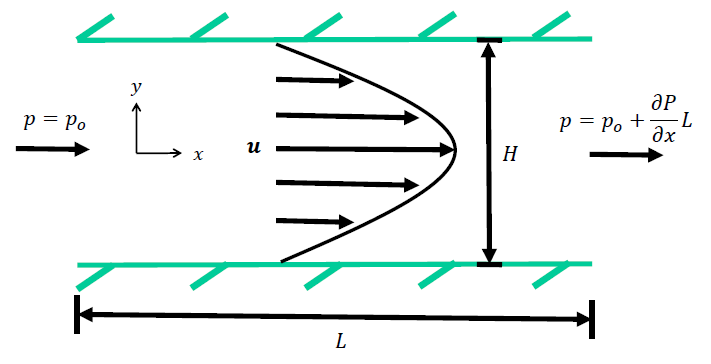
\includegraphics[width=\linewidth]{figs/poise-schematic}
    \caption{Schematic of Poiseuille flow; no-slip boundary conditions are enforced at the top and bottom boundaries, and periodic boundary conditions are enforced at the left and right boundaries.
The size of the domain is $L = 32$  and $H = 64$.}
    \label{fig:poise-schematic}
\end{figure}

Unless otherwise stated, all of the Poiseuille flow simulations were computed on a $32 \times 64$ lattice for 25000 time steps.
The lattice size was chosen to be sufficiently fine for accuracy and the number of time steps was set high enough to ensure a steady state would be reached.
In reference to computational time, each of the simulations in this section was run on a single core of an Intel I7-860 Quad-Core 2.80GHz processor.

The Bingham plastic simulations were carried out with a pressure gradient of $\pgrad = 1.0 \times 10^{-5}$, and a plastic viscosity of $\mu_p = 0.2$.
The yield stress was varied between four different values $\tau_y = \begin{bmatrix}4.0,&8.0,&12.0,&16.0\end{bmatrix} \times 10^{-5}$, and five different LBM schemes were used: (1) BGK with $m = 10^5$, (2) BGK with $m = 10^8$, (3) BGK with $m = 10^8$ and the median filter, (4) MRT-1 with $m = 10^8$, and (5) MRT-2 with $m = 10^8$.
The MRT-1 and MRT-2 schemes differ in their choice of free parameters for the relaxation matrix.
For the MRT-1 relaxation matrix, the free parameters were set to $s_1 = s_2 = s_4 = s_6 = 1.1$, which follows the recommendation of~\cite{lallemand2000theory} for reasons of stability, and has been successfully used to simulate non-Newtonian flow in the past~\cite{fallah2012multiple,grasinger2015simulation}. 
For the MRT-2 relaxation matrix, the free parameters were set to $s_1 = 1.1$, $s_2 = 1.0$, and $s_4 = s_6 = 1.2$, as these values have been successfully applied to simulating lid-driven cavity flow of non-Newtonian fluids in the past~\cite{chen2014simulations,li2014simulation}.
Additionally, in regards to the LBM schemes, recall that $m$ is the stress growth exponent for the Papanastasiou approximation, and the higher $m$ is the closer the approximation is to the true Bingham plastic behavior.
The relative $L_2$ and relative $L_{\infty}$ errors with respect to the analytical solution were computed for each simulation.
The analytical solution for Poiseuille flow of a Bingham plastic fluid is given by:
\begin{equation} \label{eq:analytical-bingham}
u_x(y) = \begin{cases}
\frac{1}{2 \mu_p} \left(-\pgrad\right) \left[h^2 - y_{\tau}^2 \right] - \frac{\tau_y}{\mu_p} \left(h - y_{\tau}\right), & 0 \leq |y| \leq y_{\tau}, \\
\frac{1}{2 \mu_p} \left(-\pgrad\right) \left[h^2 - y^2 \right] - \frac{\tau_y}{\mu_p} \left(h - |y|\right), & y_{\tau} < |y| \leq h,
\end{cases}
\end{equation}
\noindent where $y_{\tau} = -\tau_y / \pgrad$ is the vertical location at which the fluid yields.
(Note that the analytical solution is based on the exact Bingham plastic model, and not the Papanastasiou approximation.
The choice was made to compare with the analytical solution for a Bingham plastic, instead of an analytical solution or benchmark for the Papanastasiou constitutive approximation, because the Bingham plastic constitutive behavior is the behavior of interest. In addition, if the error was calculated with respect to the solution or approximation for the Papanastasiou constitutive approximation, then collision schemes with different stress growth exponents would have their error computed with respect to different solutions. Thus, it would be difficult to compare the relative errors between collision schemes. Lastly, note that although the errors computed with the respect to the Bingham plastic analytical solution do contain error in the constitutive relation, it can be seen from the accuracy of the MRT collision scheme, and others, that the constitutive relation error is likely negligible compared to other sources of error.)

The relative $L_2$ error, relative $L_{\infty}$ error, and computation time for each simulation are presented in \Fref{tab:poise-bing}.
The Reynold's number was computed by $Re = \frac{\rho U H}{\mu_p}$, where $U$ is the maximum velocity given by the analytical solution.
The Bingham number was computed by $Bn = \frac{\tau_y H}{\mu_p U}$.

\begin{table}
\centering
\caption{Bingham plastic Poiseuille flow}
\vspace{0.5cm}
\begin{tabulary}{\linewidth}{l l r r r r r r r r}
\pbox{20cm}{Collision \\ Operator} & \pbox{20cm}{Median \\ Filter} & $m$ & \pbox{20cm}{$\tau_y$ \\ $(\times 10^{-5})$} & $Re$ & $Bn$ & $L_2$ & $L_\infty$ & \pbox{20cm}{Time \\ (sec)} \\
\hline \\
BGK & No & $10^5$ & 4.0 & 6.05 & 0.68 & 0.0062 & 0.0153 & 1857 \\
& & & 8.0 & 4.42 & 1.85 & 0.0204 & 0.0411 & 2329 \\
& & & 12.0 & 3.04 & 4.04 & 0.0503 & 0.0891 & 3345 \\
& & & 16.0 & 1.92 & 8.52 & 0.1161 & 0.1879 & 2029 \\
\\
BGK & No & $10^8$ & 4.0 & 6.05 & 0.68 & 0.0109 & 0.0282 & 2831 \\
& & & 8.0 & 4.42 & 1.85 & 0.0330 & 0.0670 & 3509 \\
& & & 12.0 & 3.04 & 4.04 & 0.0788 & 0.1570 & 4838 \\
& & & 16.0 & 1.92 & 8.52 & 0.1991 & 0.3539 & 3790 \\
\\
BGK & Yes & $10^8$ & 4.0 & 6.05 & 0.68 & 0.0100 & 0.0273 & 2903 \\
& & & 8.0 & 4.42 & 1.85 & 0.0361 & 0.0823 & 3567 \\
& & & 12.0 & 3.04 & 4.04 & 0.2439 & 0.3832 & 4800 \\
& & & 16.0 & 1.92 & 8.52 & 0.7533 & 1.0718 & 3507 \\
\\
MRT-1 & No & $10^8$ & 4.0 & 6.05 & 0.68 & 0.0013 & 0.0013 & 5914 \\
& & & 8.0 & 4.42 & 1.85 & 0.0018 & 0.0018 & 7908 \\
& & & 12.0 & 3.04 & 4.04 & 0.0026 & 0.0026 & 7160 \\
& & & 16.0 & 1.92 & 8.52 & 0.0041 & 0.0041 & 5559 \\
\\
MRT-2 & No & $10^8$ & 4.0 & 6.05 & 0.68 & 0.0012 & 0.0012 & 5284 \\
& & & 8.0 & 4.42 & 1.85 & 0.0017 & 0.0017 & 5290 \\
& & & 12.0 & 3.04 & 4.04 & 0.0024 & 0.0024 & 5244 \\
& & & 16.0 & 1.92 & 8.52 & 0.0038 & 0.0038 & 4532 \\
\\
\label{tab:poise-bing}
\end{tabulary}
\end{table}

As has been reported previously, for the BGK collision operator, using a stress growth exponent of $m = 10^5$ is more accurate with respect to the analytical solution than using a stress growth exponent of $m = 10^8$~\cite{chen2014simulations}.
A larger stress growth exponent results in a more accurate Papastasiou approximation of the true Bingham plastic constitutive model, however, it leads to more nonphysical oscillations that degrade the numerical solution for the BGK collision operator.
Upon inspection of \Fref{tab:poise-bing}, it does not appear that entropic median filtering helped to mitigate errors that occurred as a result of using $m = 10^8$ for Bingham plastic Poiseuille flow.
In fact, the median filter resulted in a less accurate solution in all cases other than the case with the lowest yield stress considered (i.e., the smoothest flow field), and rendered the solution altogether useless for the higher yield stress fluids (relative errors of approximately 25--75\%).

In general, the BGK collision operator using a stress growth exponent of $m = 10^5$ had the lowest computational time.
This can be attributed to the fact that a smoother approximation of the Bingham plastic constitutive model would lead to a solution for $\mu_{app}$ converging with less iterations.
The BGK collision operator using a stress growth exponent of $m = 10^5$ experienced relatively low error for lower yield stress fluids, however, for $\tau_y = 12 \times 10^{-5}$ and $16 \times 10^{-5}$ the relative $L_\infty$ errors were 8.9\% and 19\%, respectively, which is larger than what would be considered acceptable for most engineering applications.

The LBM approximations of the velocity profile across the channel (more specifically, $u_x(\pos_j, 25000)$ where $\pos_j = \begin{Bmatrix}16 & y_j\end{Bmatrix}^T$ for $j = 1, 2, ..., 64$, i.e. $\pos_j$ is taken at 16 nodes in from the left in the x-direction and for the full height of the channel in the y-direction) for the BGK collision operator using $m = 10^5$ and $m = 10^8$ are plotted with the analytical solution \eqref{eq:bingham} in \Fref{fig:bing-analyt-bgk-5} and \Fref{fig:bing-analyt-bgk-8}, respectively.
Due to the smoothness of the LBM approximation in \Fref{fig:bing-analyt-bgk-5}, one can conclude that the error for the BGK model with $m = 10^5$ is not due to nonphysical oscillations, but instead the inaccuracy of the Papastasiou approximation with a lower stress growth exponent.
In contrast, the LBM approximation in \Fref{fig:bing-analyt-bgk-8} is not smooth, which suggests that the error for the BGK model with $m = 10^8$ is due to nonphysical oscillations. (Note: the velocity for the BGK model with $m = 10^8$ may appear asymmetric, but that is because the flow does not reach a steady-state and \Fref{fig:bing-analyt-bgk-8} is merely a snapshot in time.
The oscillations in the velocity tend to move back and forth across the channel in subsequent time steps such that, on average (in time), the oscillations are indeed symmetric.)

\begin{figure}
\centering
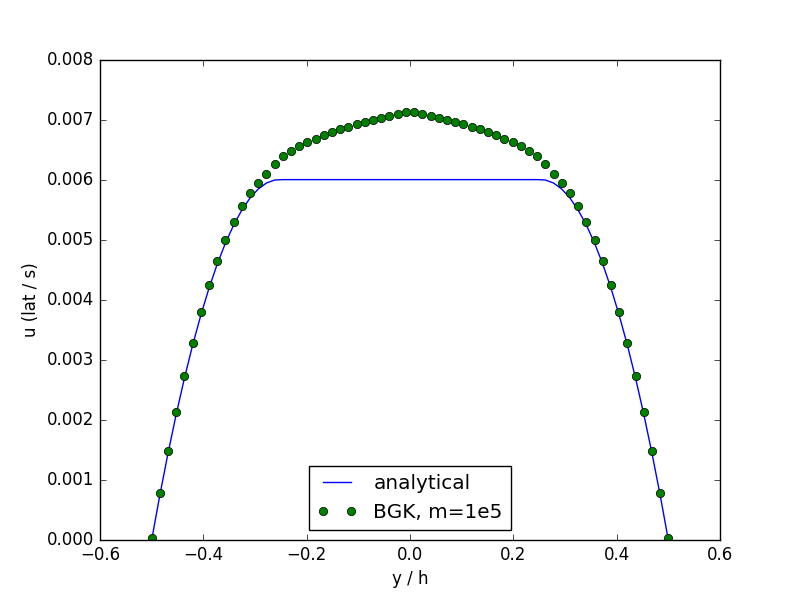
\includegraphics[width=\linewidth]{figs/poise-bingham/bgk-5/analytical-vs-approx.png}
\caption{LBM approximation using BGK and $m = 10^5$ compared to the analytical solution for $\tau_y = 16 \times 10^{-5}$.}
\label{fig:bing-analyt-bgk-5}
\end{figure}

\begin{figure}
	\centering
    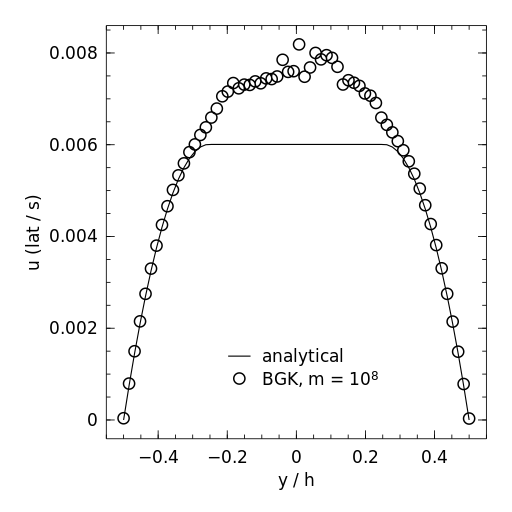
\includegraphics[width=\linewidth]{figs/poise-bingham/bgk-8/analytical-vs-approx.png}
    \caption{LBM approximation using BGK and $m = 10^8$ compared to the analytical solution for $\tau_y = 16 \times 10^{-5}$.}
\label{fig:bing-analyt-bgk-8}
\end{figure}

In order to better understand why median filtering did not eliminate the nonphysical oscillations in high yield stress fluids, but instead exacerbated the problem, it is necessary to investigate what is happening at the particle distribution scale.
\Fref{fig:feq-vs-f_bgk} compares particle distributions to quasiequilibrium.
More specifically, \Fref{fig:feq-vs-f_bgk} compares $f_i(\pos_j, 25000)$ to $f_i^{eq}(\pos_j, 25000)$ where $\pos_j = \begin{Bmatrix}16 & y_j\end{Bmatrix}^T$ for $j = 1, 2, ..., 64$, and $i = 5, 8$.
It can be seen that in the BGK, $m = 10^8$ solution, that nonphysical oscillations pollute the quasiequilibrium profile as well.
These nonphysical oscillations likely originate at the lattice scale due to the sharp gradient in the macroscopic velocity, $\mvel$, near the walls, and the sharp gradient in $\mvel$ is a result of a sharp gradient in $\mu_{app}$, namely the sharp gradient of the constitutive relationship.
Because the nonphysical oscillations make their way into the quasiequilibrium values, entropic median filtering does not help dampen the oscillations but instead contracts the particle distributions closer to the quasiequilibrium oscillations, which explains why the median filtered results were less accurate for Bingham plastic Poiseuille flow.
In order to ensure that this phenomenon was a side effect of all entropic filtering, and not just entropic median filtering with $\theta = 1.0 \times 10^{-6}$ and $n_s = 2.7$, optimization was used to find the value of $\theta$ that minimized error for both median filtering and Ehrenfests' regularization.
The optimization problem was defined as follows:
\begin{align*}
  \min_\theta \hspace{0.2in} & f(\theta)\\
  \text{such that} \hspace{0.2in} & \theta \in \begin{bmatrix}10^{-10}, & 2.0\end{bmatrix}
\end{align*}
\noindent where $f(\theta) \equiv $ the relative $L_2$ error between the LBM approximation using $m = 10^8$ and entropic filtering with a $\Delta S$ threshold of $\theta$ (used in the criteria defined in \eqref{eq:ds-threshold}).
The bounds on $\theta$, namely $\theta \in \begin{bmatrix}10^{-10}, & 2\end{bmatrix}$ represent $\theta$ such that 100\% of lattice sites are filtered for every time step ($\theta = 10^{-10}$) and $\theta$ such that no lattice sites are filtered for any time step ($\theta = 2.0$).
The optimization problem was solved for the cases of using median filtering and Ehrenfests' regularization using both Brent's method and the Golden Section search.
For all four cases, the optimal solution was $\theta = 2.0$ and the cost function, $f(2.0)$, was equal to the relative $L_2$ error for the BGK collision operator, $m = 10^8$ and no entropic filtering.
The results of the optimization show that entropic filtering, at best, did not affect the accuracy of LBM; and often adversely affected the accuracy of LBM in approximating Bingham plastic Poiseuille flow, regardless of whether median filtering or Ehrenfests' regularization was used, and regardless of what the $\Delta S$ threshold, $\theta$, was set to.

\newcommand{\figwid}{0.48\linewidth}

%MG: reformat these images so that text is more readable
\begin{figure}
\centering
\begin{tabulary}{\linewidth}{c c}
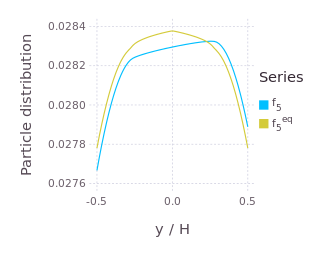
\includegraphics[width=\figwid]{figs/poise-bingham/bgk-5/feq-vs-f_5.png}
&
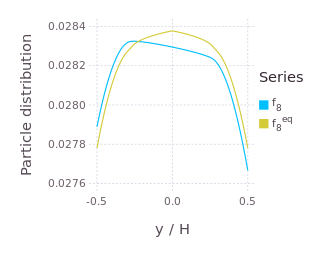
\includegraphics[width=\figwid]{figs/poise-bingham/bgk-5/feq-vs-f_8.png}
\\
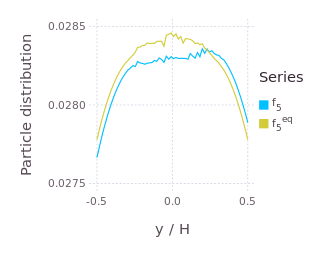
\includegraphics[width=\figwid]{figs/poise-bingham/bgk-8/feq-vs-f_5.png}
&
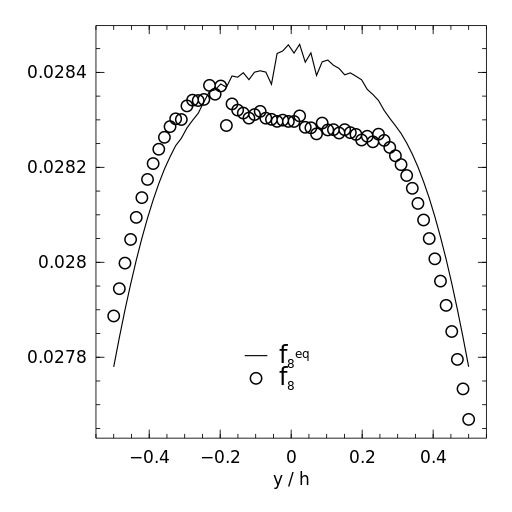
\includegraphics[width=\figwid]{figs/poise-bingham/bgk-8/feq-vs-f_8.png}
\end{tabulary}
\caption{Particle distributions in the 5 direction (left) and 8 direction (right) compared to their respective quasiequilibriums. The top two plots are for the BGK with $m = 10^5$, the bottom two are for the BGK with $m = 10^8$.}
\label{fig:feq-vs-f_bgk}
\end{figure}

On average, the LBM model using the MRT-1 collision operator took 2.9 times more computing time than the BGK collision operator with $m = 10^5$; and the model using MRT-2 took 2.1 times more computing time than the BGK collision operator with $m = 10^5$.
However, the increased computing time can be justified for the MRT collision operator because the MRT solutions did not suffer from the same level of nonphysical oscillations as the BGK collision operator when using the more accurate approximation of the Bingham plastic model, i.e. when $m = 10^8$. 
The MRT collision schemes were, therefore, the most accurate solutions for all cases; and because the difference in accuracy between the MRT-1 and MRT-2 collision schemes was negligible, the remainder of the discussion in this section will focus on comparing the BGK collision schemes and the MRT-1 collision scheme.
\Fref{fig:feq-vs-f_mrt} compares particle distribution, $f_i$, profiles to their respective quasiequilibrium profiles, $f_i^{eq}$ for the MRT-1 model.
In contrast to the BGK with $m = 10^8$, there were no significant nonphysical oscillations in the quasiequilibrium distributions.

\begin{figure}
	\centering
    \begin{tabulary}{\linewidth}{c c}
        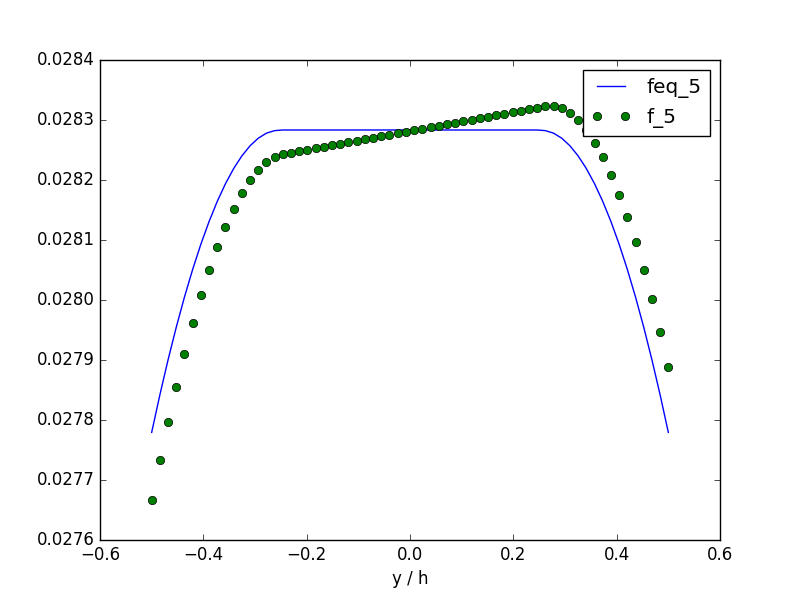
\includegraphics[width=\figwid]{figs/poise-bingham/mrt/feq-vs-f_5.png}
        &
        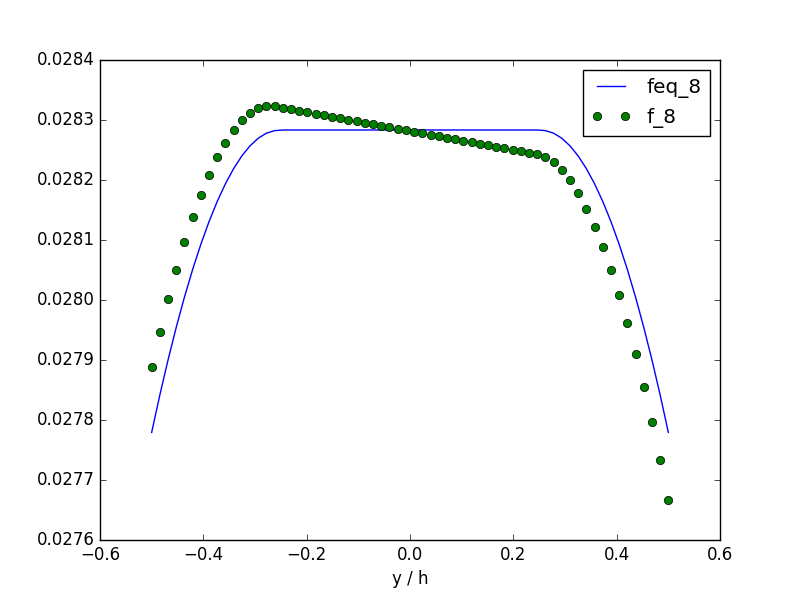
\includegraphics[width=\figwid]{figs/poise-bingham/mrt/feq-vs-f_8.png}
    \end{tabulary}
    \caption{Particle distributions in the 5 direction (left) and 8 direction (right) compared to their respective quasiequilibriums for the MRT-1 with $m = 10^8$.}
    \label{fig:feq-vs-f_mrt}
\end{figure}

Another important question to ask is, if the strength of the MRT collision operator is damping out the ghost modes, then are the nonphysical oscillations for the BGK with $m = 10^8$ (with and without median filtering) a result of the ghost modes?
\Fref{fig:epsilon} shows a measure of the nonequilibrium $\epsilon$ moment, $\boldsymbol{\epsilon}^{neq}$, with respect to time for each of the collision schemes, which was calculated as:
\begin{equation}
\frac{||\boldsymbol{\epsilon} - \boldsymbol{\epsilon}^{eq}||_2}{||\boldsymbol{\epsilon}^{eq}||_2}
\end{equation}
\noindent where $||.||_2$ is the Euclidean norm, $\epsilon_j = 4f_0(\pos_j) - 2f_1(\pos_j) - 2f_2(\pos_j) - 2f_3(\pos_j) - 2f_4(\pos_j) + f_5(\pos_j) + f_6(\pos_j) + f_7(\pos_j) + f_8(\pos_j)$ is related to the square of the energy, and $\pos_j = \begin{Bmatrix}16 & y_j\end{Bmatrix}^T$ for $j = 1, 2, ..., 64$, i.e. $\pos_j$ is taken at 16 nodes in from the left in the x-direction and for the full height of the channel in the y-direction.
The values measured for the BGK with $m = 10^8$, with and without median filtering, were significantly higher than for either the MRT-1 or BGK with $m = 10^5$ collision schemes, which suggests that the nonphysical oscillations the BGK with $m = 10^8$ displayed was in part due to the $\epsilon$ moment.

\begin{figure}
	\centering
    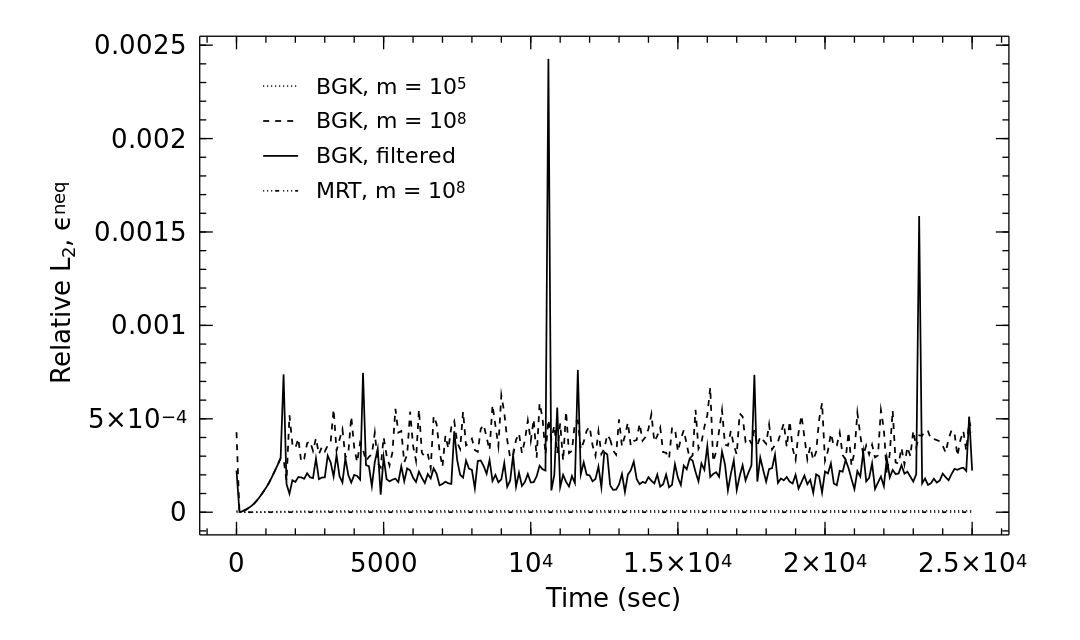
\includegraphics[width=\linewidth]{figs/poise-bingham/epsilon}
    \caption{Evolution of relative $L_2$ norm, $\epsilon^{neq}$ with time. The norm of the $\epsilon^{neq}$ across the height of the channel is an indicator of an increase in oscillations at the lattice level due to the $\epsilon$ moment.}
    \label{fig:epsilon}
\end{figure}

\Fref{fig:qx} shows a measure of the nonequilibrium $q_x$ moment, $\mathbf{q_x}^{neq}$, or energy flux in the x-direction, with respect to time for each of the collision schemes, which was calculated as:
\begin{equation}
    \frac{||\mathbf{q_x} - \mathbf{q_x}^{eq}||_2}{||\mathbf{q_x}^{eq}||_2}
\end{equation}
\noindent where $q_{x_j} = - 2f_1(\pos_j) + 2f_3(\pos_j) + f_5(\pos_j) - f_6(\pos_j) - f_7(\pos_j) + f_8(\pos_j)$ and $\pos_j$ were taken across the height of the channel in the same manner as with the $\epsilon$ moment.
The values measured for the BGK with $m = 10^8$ and median filtered were consistently greater than any other collision scheme.
The relative $L_2$ norm of the $\mathbf{q_x}^{neq}$ for the BGK collision operator with $m = 10^8$ and median filtering solution spent most of the simulation between approximately 50\% and 100\%, suggesting that the $q_x$ moment was likely the cause of the nonphysical oscillations and error in the solution.
As expected (if the dominant source of error in the LBM approximation for Bingham plastic Poiseuille flow is indeed due to the $q_x$ moment), the $\mathbf{q_x^{neq}}$ relative $L_2$ norm for the BGK with $m = 10^8$ was slightly greater than the BGK with $m = 10^5$, and the $\mathbf{q_x^{neq}}$ relative $L_2$ norm was negligible for the MRT-1 collision scheme.

\begin{figure}
	\centering
    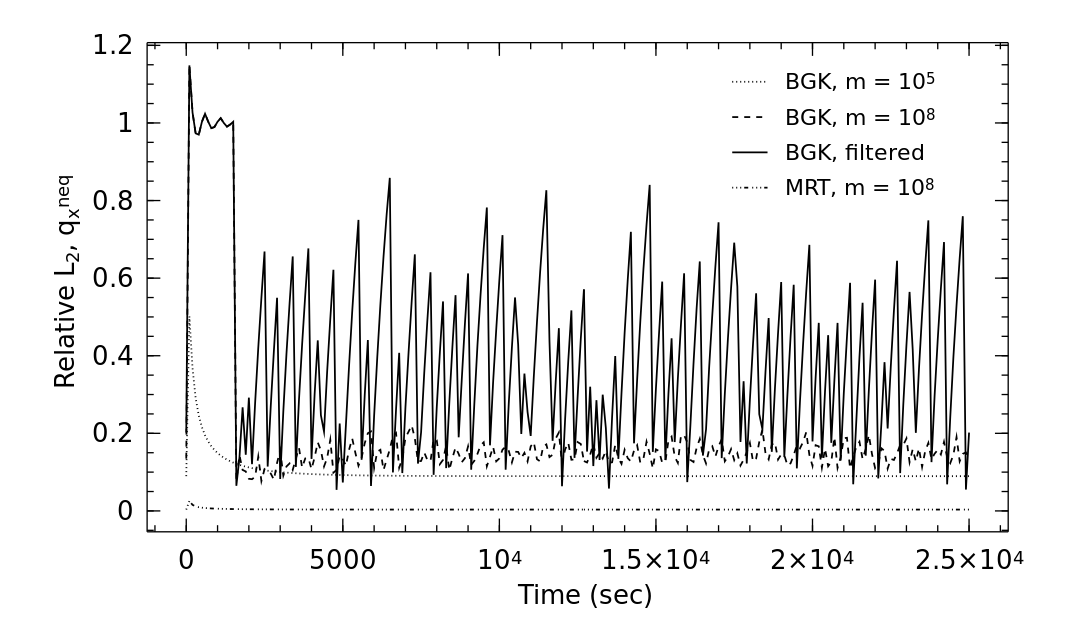
\includegraphics[width=\linewidth]{figs/poise-bingham/qx}
    \caption{Evolution of relative $L_2$ norm, $\mathbf{q_x}^{neq}$ with time. The norm of the $\mathbf{q_x^{neq}}$ across the height of the channel is an indicator of an increase in oscillations at the lattice level due to the $q_x$ moment.}
    \label{fig:qx}
\end{figure}

It is likely that the nonequilibrium $\epsilon$ and $q_x$ moments cause nonphysical oscillations in particle distributions, $f_i$, with a cumulative effect in time (i.e. oscillations build in amplitude with time).
\Fref{fig:epsilon-cumulative} and \Fref{fig:qx-cumulative} show the cumulative measures of the nonequilibrium moments in time, which was calculated, respectively, as:
\begin{equation}
  \int_0^{T} \frac{||\boldsymbol{\epsilon}(t) - \boldsymbol{\epsilon}^{eq}(t)||_2}{||\boldsymbol{\epsilon}^{eq}(t)||_2} dt,
\end{equation}
\noindent and,
\begin{equation}
  \int_0^{T} \frac{||\mathbf{q_x}(t) - \mathbf{q_x}^{eq}(t)||_2}{||\mathbf{q_x}^{eq}(t)||_2} dt,
\end{equation}
\noindent where $T$ is the current time. 
\Fref{fig:qx} and \Fref{fig:qx-cumulative} show that both the peak and cumulative values of the relative $L_2$ norm of $\mathbf{q_x}^{neq}$ are much larger than the peak and cumulative values of the relative $L_2$ norm of $\boldsymbol{\epsilon}^{neq}$, which suggests that the ghost mode associated with the $q_x$ moment dominates and is the primary source of oscillations.
It can be inferred that the $q_x$ moment was a significant source of oscillations in this case because the Poiseuille flow was in the x-direction.
Overall, the results presented suggest that if an LBM collision scheme is to be developed for simulating high yield stress, Poiseuille-type flow that is more accurate than the BGK with $m = 10^5$ and more computationally efficient than the MRT, it should focus on a means of dampening the nonequilibrium energy flux moments, namely $q_x$ and $q_y$.

\begin{figure}
    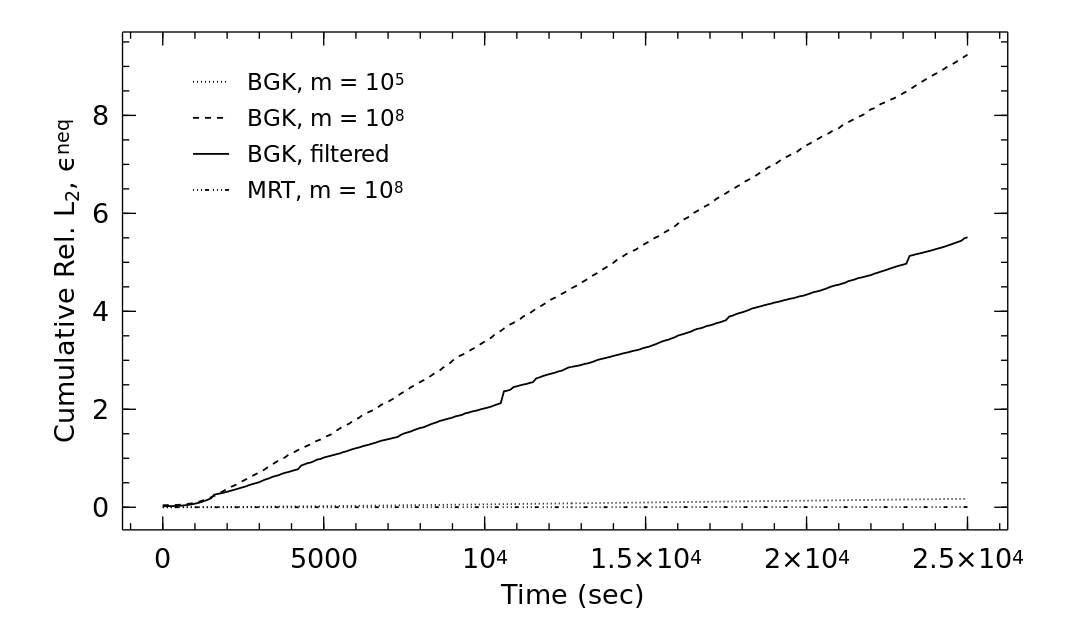
\includegraphics[width=\linewidth]{figs/poise-bingham/epsilon_cumulative}
    \caption{Cumulative relative $L_2$ norm, $\epsilon^{neq}$ with time. Oscillations can have a positive effect on each other. The cumulative relative $L_2$, $\epsilon^{neq}$ is a measure of how much oscillations due to the $\epsilon$ moment may have been building in time.}
    \label{fig:epsilon-cumulative}
\end{figure}

\begin{figure}
    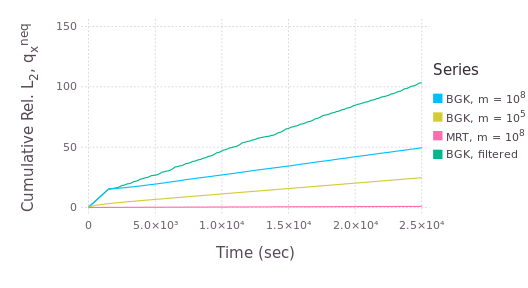
\includegraphics[width=\linewidth]{figs/poise-bingham/qx_cumulative}
    \caption{Cumulative relative $L_2$ norm, $\mathbf{q_x^{neq}}$ with time. Oscillations can have a positive effect on each other. The cumulative relative $L_2$, $\mathbf{q_x^{neq}}$ is a measure of how much oscillations due to the $q_x$ moment may have been building in time.}
    \label{fig:qx-cumulative}
\end{figure}

Lastly, simulations with the same collision schemes, Reynold's numbers, and Bingham numbers were run on $128 \times 32$ lattices in order to investigate the effect of grid resolution.
The plastic viscosity was held constant ($\mu_p = 0.2$.), while the yield stress and pressure gradient were varied in order to match the Reynold's numbers and Bingham numbers in \Fref{tab:poise-bing}.
The relative $L_2$ error, relative $L_{\infty}$ error, and computation time for each simulation are presented in \Fref{tab:poise-bing-2}.

As would be expected from doubling the number of lattice sites, the cost for each corresponding combination of collision scheme, $Re$, and $Bn$ increased by a factor of approximately 2--2.5.
The 2--2.5 times increase in computing time resulted in the BGK collision schemes on the finer lattice being comparable in computational cost to the MRT collision schemes on the coarser lattice.
In regards to error, for the larger Bingham number flows ($Bn = 4.04, 8.52$) both the $L_2$ and $L_\infty$ errors of the BGK collision schemes were reduced in general, sometimes by as much as a factor of 4.
None of the relative $L_2$ errors exceeded 10\%, in contrast to the BGK simulations run on the coarser lattice.
However, despite the increase in accuracy, it should be noted that for $Bn = 8.52$ all of the BGK collision schemes had $L_\infty$ errors that exceeded 10\%.
The MRT collision schemes, even on the coarser lattice, were more accurate (for the case of $Bn = 8.52$) than all of the BGK collision schemes on the finer lattice.
Again, the difference in the accuracies between the MRT-1 and MRT-2 collision schemes appears to be negligible.
The difference in computational cost is also low, though the MRT-2 collision scheme took 4\% less computing time on average.

\begin{table}
	\centering
	\caption{Bingham plastic Poiseuille flow, $128 \times 32$ lattice}
	\vspace{0.5cm}
	\begin{tabulary}{\linewidth}{l l r r r r r r r r}
		\pbox{20cm}{Collision \\ Operator} & \pbox{20cm}{Median \\ Filter} & $m$ & \pbox{20cm}{$\tau_y$ \\ $(\times 10^{-5})$} & $Re$ & $Bn$ & $L_2$ & $L_\infty$ & \pbox{20cm}{Time \\ (sec)} \\
		\hline \\
		BGK & No & $10^5$ & 1.0 & 6.05 & 0.68 & 0.0419 & 0.0450 & 4951 \\
		              & & & 2.0 & 4.42 & 1.85 & 0.0300 & 0.0370 & 5209 \\
	                  & & & 3.0 & 3.04 & 4.04 & 0.0206 & 0.0260 & 5296 \\
		              & & & 4.0 & 1.92 & 8.52 & 0.0649 & 0.1016 & 5304 \\
		\\
		BGK & No & $10^8$ & 1.0 & 6.05 & 0.68 & 0.0426 & 0.0470 & 6484 \\
		              & & & 2.0 & 4.42 & 1.85 & 0.0306 & 0.0394 & 7111 \\
		              & & & 3.0 & 3.04 & 4.04 & 0.0230 & 0.0438 & 7595 \\
		              & & & 4.0 & 1.92 & 8.52 & 0.0963 & 0.1659 & 7791 \\
		\\
		BGK & Yes & $10^8$ & 1.0 & 6.05 & 0.68 & 0.0427 & 0.0468 & 5576 \\
		               & & & 2.0 & 4.42 & 1.85 & 0.0309 & 0.0397 & 7512 \\
		               & & & 3.0 & 3.04 & 4.04 & 0.0236 & 0.0443 & 7856 \\
		               & & & 4.0 & 1.92 & 8.52 & 0.0934 & 0.1624 & 7848 \\
		\\
		MRT-1 & No & $10^8$ & 1.0 & 6.05 & 0.68 & 0.0452 & 0.0484 & 13837 \\
		              & & & 2.0 & 4.42 & 1.85 & 0.0404 & 0.0435 & 16515 \\
                      & & & 3.0 & 3.04 & 4.04 & 0.0316 & 0.0338 & 17142 \\
                      & & & 4.0 & 1.92 & 8.52 & 0.0197 & 0.0210 & 17853 \\
		\\
		MRT-2 & No & $10^8$ & 1.0 & 6.05 & 0.68 & 0.0453 & 0.0485 & 14030 \\
		& & & 2.0 & 4.42 & 1.85 & 0.0404 & 0.0435 & 15290 \\
		& & & 3.0 & 3.04 & 4.04 & 0.0316 & 0.0338 & 16328 \\
		& & & 4.0 & 1.92 & 8.52 & 0.0198 & 0.0210 & 16816 \\
		\\
		\label{tab:poise-bing-2}
	\end{tabulary}
\end{table}

\subsection{Lid-driven Cavity Flow} % MG: would it be of any use to show streamline plots from some of these flows?

A lid-driven benchmark problem was chosen for this numerical study because there are many results available in literature in which to compare with and because the vorticity of the flow coupled with the nonlinear constitutive equations should result in a challenge in terms of stability.
As was done herein, lid-driven cavity flow is generally characterized by a square cavity where a fluid velocity is prescribed tangential to the upper boundary and the remaining boundaries have a no-slip boundary condition.
The example of lid-driven cavity flow utilized herein is presented schematically in \Fref{fig:lid-driven}.

\begin{figure}
\centering
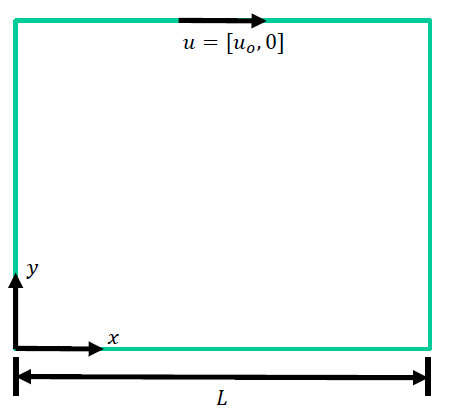
\includegraphics{figs/lid-driven}
\caption{Schematic of lid-driven cavity flow; a velocity is prescribed tangential to the top boundary and no-slip is enforced at the remaining boundaries. $L = 100$}
\label{fig:lid-driven}
\end{figure}

Unless specified otherwise, the lid-driven cavity simulations presented in the section were all simulated on a relatively coarse, $100 \times 100$ lattice, similar to the work presented in ~\cite{brownlee2008nonequilibrium}.
A coarse lattice was chosen in order to highlight concerns with stability and accuracy.
The simulations were run for either 50000 time steps or until convergence was met.
Convergence was defined by:
\begin{equation} \label{eq:convergence}
\sum_{m=1}^{100} \sum_{i, j} \frac{|u_{i, j}^k - u_{i, j}^{k-m}|}{|u_{i, j}^{k-m}|} < 1.0 \times 10^{-7},
\end{equation}
\noindent where $i$ is the node index in the x-direction, $j$ is the node index in the y-direction, and $k$ is the current time step.
The lid velocity was prescribed as $u_o = 0.1$.
All coordinate values presented in this section (used to describe the location of the center of vortices) are given normalized with respect to the length of the cavity side (i.e. as $(x / L, y / L)$).
Note that all results presented as ``-'' indicate that the tests were numerically unstable to the extent that the degrees of freedom all over the domain were diverging toward $-\infty$ or $\infty$.

\subsubsection{Bingham Plastic Fluids}

For the Bingham plastic numerical tests the Reynold's number was varied with the following values: $\begin{bmatrix}100,&1000,&5000,&10000\end{bmatrix}$, and the Bingham number was varied with the following values: $\begin{bmatrix}1,&10,&100\end{bmatrix}$ ($Bn$ and $Re$ were calculated the same as in \Fref{sec:poise-bing}).
Six collision schemes were tested: (1) BGK with $m = 10^5$, (2) BGK with $m = 10^8$, (3) BGK-BRT with $m = 10^8$, (4) BGK with $m = 10^8$ and median filtering, (5) MRT with $m = 10^8$ and (6) MRT with $m = 10^8$ and median filtering.
For the MRT relaxation matrix, the free parameters were set to $s_1 = 1.1$, $s_2 = 1.0$, and $s_4 = s_6 = 1.2$ (same as MRT-2 in \Fref{sec:poise-bing}).
Tables \ref{tab:lid-bing1}--\ref{tab:lid-bing100} compare the center location of the main vortex to literature values taken from~\citet{syrakos2014performance}.
The main vortex location is determined by calculating the stream function using Simpson's rule and finding where it attains a maximum.

\begin{table}
\centering
\caption{Bingham plastic, lid-driven cavity flow; $Bn = 1$.}
\small
\vspace{0.5cm}
\begin{tabulary}{\linewidth}{r r l l r r r r}
$Bn$ & $Re$ & \pbox{20cm}{Collision \\ Operator} & \pbox{20cm}{Median \\ Filter} & $m$ & \pbox{20cm}{Vortex \\ Center \\ (literature)} &  \pbox{20cm}{Vortex \\ Center \\ (LBM)} & \pbox{20cm}{Time \\ (sec)} \\
\hline \\
1 & 100 & BGK     & No  & $10^5$ & (0.63, 0.79) & (0.63, 0.79) & 17685 \\
  &     & BGK     & No  & $10^8$ &              & (0.63, 0.79) & 19398 \\
  &     & BGK-BRT & No  & $10^8$ &              & (0.63, 0.79) & 22656 \\
  &     & BGK     & Yes & $10^8$ &              & (0.63, 0.79) & 21535 \\
  &     & MRT     & No  & $10^8$ &              & (0.63, 0.79) & 79040 \\
  &     & MRT     & Yes & $10^8$ &              & (0.63, 0.79) & 85295 \\
\\
1 & 1000 & BGK     & No  & $10^5$ & (0.54, 0.57) & (0.54, 0.57) & 16109 \\
  &      & BGK     & No  & $10^8$ &              & (0.54, 0.57) & 17035 \\
  &      & BGK-BRT & No  & $10^8$ &              & (0.54, 0.57) & 16879 \\
  &      & BGK     & Yes & $10^8$ &              & (0.54, 0.57) & 20170 \\
  &      & MRT     & No  & $10^8$ &              & (0.54, 0.57) & 46048 \\
  &      & MRT     & Yes & $10^8$ &              & (0.54, 0.57) & 55818 \\
\\
1 & 5000 & BGK     & No  & $10^5$ & (0.52, 0.53) & - & - \\
  &      & BGK     & No  & $10^8$ &              & - & - \\
  &      & BGK-BRT & No  & $10^8$ &              & - & - \\
  &      & BGK     & Yes & $10^8$ &              & (0.54, 0.53) & 17248 \\
  &      & MRT     & No  & $10^8$ &              & (0.51, 0.55) & 50572 \\
  &      & MRT     & Yes & $10^8$ &              & (0.52, 0.53) & 54225 \\
\\
1 & 10000 & BGK     & No  & $10^5$ & N/A          & - & - \\
  &       & BGK     & No  & $10^8$ &              & - & - \\
  &       & BGK-BRT & No  & $10^8$ &              & - & - \\
  &       & BGK     & Yes & $10^8$ &              & (0.56, 0.60) & 18186 \\
  &       & MRT     & No  & $10^8$ &              & (0.48, 0.48) & 43246 \\
  &       & MRT     & Yes & $10^8$ &              & (0.46, 0.54) & 50864 \\
\\
\end{tabulary}
\label{tab:lid-bing1}
\end{table}
\begin{table}
\centering
    \caption{Bingham plastic, lid-driven cavity flow; $Bn = 10$.}
    \small
    \vspace{0.5cm}
\begin{tabulary}{\linewidth}{r r l l r r r r}
    $Bn$ & $Re$ & \pbox{20cm}{Collision \\ Operator} & \pbox{20cm}{Median \\ Filter} & $m$ & \pbox{20cm}{Vortex \\ Center \\ (literature)} &  \pbox{20cm}{Vortex \\ Center \\ (LBM)} & \pbox{20cm}{Time \\ (sec)} \\
    \hline \\
10 & 100 & BGK     & No  & $10^5$ & (0.53, 0.87) & (0.54, 0.87) & 25217 \\
   &     & BGK     & No  & $10^8$ &              & (0.55, 0.87) & 38285 \\
   &     & BGK-BRT & No  & $10^8$ &              & (0.55, 0.87) & 29539 \\
   &     & BGK     & Yes & $10^8$ &              & (0.54, 0.87) & 35817 \\
   &     & MRT     & No  & $10^8$ &              & (0.53, 0.88) & 143741 \\
   &     & MRT     & Yes & $10^8$ &              & (0.54, 0.88) & 135059 \\
\\
10 & 1000 & BGK     & No  & $10^5$ & (0.80, 0.85) & (0.78, 0.83) & 11525 \\
   &      & BGK     & No  & $10^8$ &              & (0.78, 0.83) & 26671 \\
   &      & BGK-BRT & No  & $10^8$ &              & (0.78, 0.83) & 19248 \\
   &      & BGK     & Yes & $10^8$ &              & (0.79, 0.84) & 34143 \\
   &      & MRT     & No  & $10^8$ &              & (0.79, 0.84) & 105136 \\
   &      & MRT     & Yes & $10^8$ &              & (0.79, 0.84) & 111942 \\
\\
10 & 5000 & BGK     & No  & $10^5$ & (0.60, 0.55) & - & - \\
   &      & BGK     & No  & $10^8$ &              & - & - \\
   &      & BGK-BRT & No  & $10^8$ &              & - & - \\
   &      & BGK     & Yes & $10^8$ &              & (0.52, 0.55) & 34638 \\
   &      & MRT     & No  & $10^8$ &              & (0.55, 0.55) & 111274 \\
   &      & MRT     & Yes & $10^8$ &              & (0.55, 0.53) & 121685 \\
\\
10 & 10000 & BGK     & No  & $10^5$ & N/A          & - & - \\
   &       & BGK     & No  & $10^8$ &              & - & - \\
   &       & BGK-BRT & No  & $10^8$ &              & - & - \\
   &       & BGK     & Yes & $10^8$ &              & (0.49, 0.54) & 19351 \\
   &       & MRT     & No  & $10^8$ &              & (0.53, 0.54) & 69249 \\
   &       & MRT     & Yes & $10^8$ &              & (0.53, 0.53) & 69054 \\
\\
\end{tabulary}
\label{tab:lid-bing10}
\end{table}
\begin{table}
\centering
    \caption{Bingham plastic, lid-driven cavity flow; $Bn = 100$.}
    \small
    \vspace{0.5cm}
    \begin{tabulary}{\linewidth}{r r l l r r r r}
        $Bn$ & $Re$ & \pbox{20cm}{Collision \\ Operator} & \pbox{20cm}{Median \\ Filter} & $m$ & \pbox{20cm}{Vortex \\ Center \\ (literature)} &  \pbox{20cm}{Vortex \\ Center \\ (LBM)} & \pbox{20cm}{Time \\ (sec)} \\
        \hline \\
100 & 100 & BGK     & No  & $10^5$ & (0.51, 0.95) & (0.51, 0.95) & 13237 \\
    &     & BGK     & No  & $10^8$ &              & (0.54, 0.96) & 26782 \\
    &     & BGK-BRT & No  & $10^8$ &              & (0.53, 0.96) & 33095 \\
    &     & BGK     & Yes & $10^8$ &              & (0.58, 0.96) & 34430 \\
    &     & MRT     & No  & $10^8$ &              & (0.49, 0.95) & 161998 \\
    &     & MRT     & Yes & $10^8$ &              & (0.54, 0.96) & 162085 \\
\\
100 & 1000 & BGK     & No  & $10^5$ & (0.53, 0.95) & (0.54, 0.95) & 42233 \\
    &      & BGK     & No  & $10^8$ &              & (0.64, 0.95) & 47364 \\
    &      & BGK-BRT & No  & $10^8$ &              & (0.60, 0.92) & 46289 \\
    &      & BGK     & Yes & $10^8$ &              & (0.79, 0.95) & 48225 \\
    &      & MRT     & No  & $10^8$ &              & (0.54, 0.95) & 190119 \\
    &      & MRT     & Yes & $10^8$ &              & (0.55, 0.95) & 188242 \\
\\
100 & 5000 & BGK     & No  & $10^5$ & (0.93, 0.97) & - & - \\
    &      & BGK     & No  & $10^8$ &              & - & - \\
    &      & BGK-BRT & No  & $10^8$ &              & - & - \\
    &      & BGK     & Yes & $10^8$ &              & (0.91, 0.95) & 57354 \\
    &      & MRT     & No  & $10^8$ &              & (0.92, 0.96) & 163318 \\
    &      & MRT     & Yes & $10^8$ &              & (0.93, 0.95) & 159523 \\
\\
100 & 10000 & BGK     & No  & $10^5$ & (0.92, 0.94) & - & - \\
    &       & BGK     & No  & $10^8$ &              & - & - \\
    &       & BGK-BRT & No  & $10^8$ &              & - & - \\
    &       & BGK     & Yes & $10^8$ &              & (0.84, 0.88) & 32080 \\
    &       & MRT     & No  & $10^8$ &              & (0.89, 0.91) & 152707 \\
    &       & MRT     & Yes & $10^8$ &              & (0.89, 0.91) & 145722 \\
\\
\end{tabulary}
\label{tab:lid-bing100}
\end{table}

Just as before with the Bingham plastic Poiseuille flow, if using the BGK collision operator and entropic filtering is not available, a stress growth exponent of $m = 10^5$ yields faster and more accurate results than using a larger stress growth exponent.
A smaller stress growth exponent is also more effective at producing accurate results in the BGK collision scheme than placing bounds on the relaxation time (i.e. BGK-BRT).
However, although the BGK with $m = 10^5$ was the fastest model in all cases, it was also unstable for $Re \ge 5000$.
The collision schemes that were unstable for $Re \ge 5000$ (BGK with $m = 10^5$, BGK with $m = 10^8$, and BGK-BRT with $m = 10^8$) were run with a finer $200 \times 200$ lattice to see if increased lattice resolution could increase stability without causing a significant increase computational efficiency.
With the finer lattice, the BGK models without median filtering were numerically unstable and took 85\% to 308\% of the computational time of the corresponding $100 \times 100$ lattice MRT model.
BGK tests conducted on a $300 \times 300$ lattice with $m = 10^8$ (without entropic filtering) for Bingham numbers of $\begin{bmatrix}1,&10\end{bmatrix}$ and Reynold’s numbers of $\begin{bmatrix}5000,&10000\end{bmatrix}$ also yielded unstable results.

For flow with $Re \ge 5000$, the BGK with $m = 10^8$ and median filtering produced numerically stable results.
However, in general, the BGK with $m = 10^8$ and median filtering was consistently different from literature values. 
The apparent inaccuracy with regards to BGK with $m = 10^8$ and median filtering is probably due to how the numerical stability is enhanced through artificial, nonphysical dissipation.
In contrast to the nonphysical nature in which median filtering enhances stability, the stability enhancement used by MRT does not directly affect the macroscopic hydrodynamics of interest, so it again provides a stable, and in most of the cases examined herein, the most accurate solution.
The apparent superiority in terms of stability and accuracy of the MRT collision operator still comes at a price though.
The MRT collision operator was, in general, 5-10 times slower than any of the BGK collision schemes.
The increase in computational expense is probably not due to the collision process itself (i.e. \eqref{eq:mrt-colop}) but instead due to calculating the strain-rate \eqref{eq:srtensor-mrt} for each iteration of the solution for the apparent viscosity, $\mu_{app}$.

In summary, for the lid-driven cavity flow of a Bingham plastic fluid, 
\begin{itemize}
    \item for low Reynold's number flow the BGK collision operator with $m = 10^5$ provides an accurate solution with a relatively small amount of computing time,
    \item for high Reynold's number flow the BGK collision operator requires entropic filtering to remain stable,
    \item and the MRT collision operator with $m = 10^8$ produces solutions with high accuracy and stability for all of the cases examined herein, but at an increased (approximately 5--10 times more) computing cost.
\end{itemize} 

\subsubsection{Power-law Fluids}

For the power-law numerical tests the Reynold's number was varied with the following values: $\begin{bmatrix}100,&1000,&5000,&10000\end{bmatrix}$, and the flow behavior index, $n$, was varied with the following values: $\begin{bmatrix}0.5,&1.5\end{bmatrix}$.
The Reynold's number was calculated as $\rho \frac{U^{2-n} H^n}{k}$.
Five collision schemes were tested: (1) BGK, (2) BGK-BRT, (3) BGK with median filtering, (4) MRT and (5) MRT with median filtering.
\Fref{tab:lid-powerlaw05} and \Fref{tab:lid-powerlaw15} compare the center location of the main vortex to literature values taken from~\citet{li2014simulation}.

%MG: two values still need filled in in these tables
\begin{table}
\centering
\caption{Power-law, lid-driven cavity flow; $n = 0.5$.}
\small
\vspace{0.5cm}
\begin{tabulary}{\linewidth}{r r l l r r r}
$n$ & $Re$ & \pbox{20cm}{Collision \\ Operator} & \pbox{20cm}{Median \\ Filter} & \pbox{20cm}{Vortex \\ Center \\ (literature)} &  \pbox{20cm}{Vortex \\ Center \\ (LBM)} & \pbox{20cm}{Time \\ (sec)} \\
\hline \\
0.5 & 100 & BGK     & No  & (0.72, 0.78) & (0.71, 0.77) & 21429 \\
    &     & BGK-BRT & No  &              & (0.71, 0.77) & 14547 \\
    &     & BGK     & Yes &              & (0.72, 0.78) & 33221 \\
    &     & MRT     & No  &              & (0.71, 0.77) & 77287 \\
    &     & MRT     & Yes &              & (0.71, 0.77) & 110403 \\
\\
0.5 & 1000 & BGK     & No  & (0.58, 0.55) & - & - \\
    &      & BGK-BRT & No  &              & - & - \\
    &      & BGK     & Yes &              & (0.53, 0.59) & 24935 \\
    &      & MRT     & No  &              & (0.53, 0.54) & 72102 \\
    &      & MRT     & Yes &              & (0.53, 0.54) & 78300 \\
\\
0.5 & 5000 & BGK     & No  & (0.53, 0.52) & - & - \\
    &      & BGK-BRT & No  &              & - & - \\
    &      & BGK     & Yes &              & (0.63, 0.68) & 23517 \\
    &      & MRT     & No  &              & - & - \\
    &      & MRT     & Yes &              & (0.51, 0.58) & 54225 \\
\\
0.5 & 10000 & BGK     & No  & (0.53, 0.52) & - & - \\
    &       & BGK-BRT & No  &              & - & - \\
    &       & BGK     & Yes &              & (0.50, 0.55) & 22603 \\
    &       & MRT     & No  &              & - & - \\
    &       & MRT     & Yes &              & (0.50, 0.54) & 63892 \\
\\
\end{tabulary}
\label{tab:lid-powerlaw05}
\end{table}

\begin{table}
\centering
\caption{Power-law, lid-driven cavity flow; $n = 1.5$.}
\small
\vspace{0.5cm}
\begin{tabulary}{\linewidth}{r r l l r r r}
$n$ & $Re$ & \pbox{20cm}{Collision \\ Operator} & \pbox{20cm}{Median \\ Filter} & \pbox{20cm}{Vortex \\ Center \\ (literature)} &  \pbox{20cm}{Vortex \\ Center \\ (LBM)} & \pbox{20cm}{Time \\ (sec)} \\
\hline \\
1.5 & 100 & BGK     & No  & (0.56, 0.73) & (0.57, 0.73) & 10897 \\
    &     & BGK-BRT & No  &              & (0.57, 0.73) & 6239 \\
    &     & BGK     & Yes &              & (0.56, 0.73) & 11847 \\
    &     & MRT     & No  &              & (0.56, 0.73) & 39017 \\
    &     & MRT     & Yes &              & (0.56, 0.73) & 96033 \\
\\
  1.5 & 1000 & BGK   & No  & (0.55, 0.64) & (0.54, 0.61) & 19764 \\
    &      & BGK-BRT & No  &                & (0.54, 0.61) & 11949 \\
    &      & BGK     & Yes &                & (0.54, 0.61) & 24516 \\
    &      & MRT     & No  &                & (0.54, 0.61) & 58714 \\
    &      & MRT     & Yes &                & (0.54, 0.61) & 69884 \\
\\
  1.5 & 5000 & BGK     & No  & (0.53, 0.61) & (0.52, 0.57) & 20147 \\
    &      & BGK-BRT & No  &              & (0.52, 0.57) & 12116 \\
    &      & BGK     & Yes &              & (0.52, 0.57) & 23140 \\
    &      & MRT     & No  &              & (0.53, 0.57) & 60584 \\
    &      & MRT     & Yes &              & (0.52, 0.58) & 58519 \\
\\
  1.5 & 10000 & BGK     & No  & (0.51, 0.55) & (0.53, 0.55) & 21570 \\
    &       & BGK-BRT & No  &              & (0.53, 0.55) & 12841 \\
    &       & BGK     & Yes &              & (0.53, 0.55) & 21570 \\
    &       & MRT     & No  &              & (0.49, 0.56) & 61453 \\
    &       & MRT     & Yes &              & (0.49, 0.55) & 67546 \\
\\
\end{tabulary}
\label{tab:lid-powerlaw15}
\end{table}

For the shear-thinning results, $n = 0.5$, at the lowest Reynold's number considered, $Re = 100$, all of the collision schemes produced results that agreed well with the literature value.
However, the solutions became unstable at higher Reynold's numbers and entropic filtering was necessary to produce a stable solution when $Re \ge 1000$ for the BGK collision operator, and when $Re \ge 5000$ for the MRT collision operator.
Although there still appears to be a tradeoff between computational efficiency and accuracy in regards to the BGK with median filtering and MRT with median filtering, it does not seem to be nearly as significant as when simulating Bingham plastic lid-driven flow (e.g. neither collision scheme consistently agrees with the literature values and the MRT with median filtering is only 2-3 times slower than the BGK with median filtering).
An example of this tradeoff is the shear-thinning results for $Re = 5000$: the location of the main vortex for the BGK with median filtering differed from the literature by more than 10\% in both the $x$ and $y$ directions, but the MRT with median filtering has approximately twice the computing cost.

For the shear-thickening results, $n = 1.5$, there were no issues of instability.
What is interesting is that all of the collision schemes produce similar results for each of the cases, with the difference in the location of the main vortex being no greater than 1\% in either the $x$ or $y$ direction for any two collision schemes (with the exception of the high Reynold's number case, $Re = 10000$).
The BGK-BRT consistently needed the least amount of computing time.
The reason the BGK-BRT may be the most efficient is because the collision frequency, $\omega$, is bounded, and consequently $\mu_{app}$ is bounded, meaning the solution to the constitutive equation may be converging with less iterations than the other collision schemes.

\section{Conclusions} \label{sec:numerical-study-conclusions}

A numerical investigation into the accuracy, stability, and efficiency of LBM collision models and stability enhancements when applied to non-Newtonian flow was presented.
The numerical investigation included testing the BGK and MRT collision operators, with and without entropic filtering, as applied to Bingham plastics and power-law fluids.
Two different benchmark problems were chosen for the study: Poiseuille flow, and lid-driven square cavity flow.
The results showed that for higher yield stress fluids in Poiseuille-type flow, only the MRT collision operator was able to use an accurate approximation to true Bingham plastic behavior and not suffer from nonphysical oscillations.
The oscillations appeared to be due to high nonequilibrium values for the moment related to the square of the energy, $\epsilon$, and the energy flux moment in the direction of flow, $q_x$.
If a collision scheme is to be developed for higher yield stress, Poiseuille-type flow that is (1) more accurate than the BGK collision operator with $m = 10^5$ and (2) more computationally efficient than the MRT collision operator, then it should focus on dampening the nonequilibrium $\epsilon$ moment and energy flux moment (in the direction of flow).

The results of the study suggest that entropic filtering can be an effective technique for enhancing stability in non-Newtonian flow, especially for high Reynold's number flows and flows that tend to produce vortices.
However, if the filter is not carefully tuned by properly adjusting the threshold or number of standard deviations then the physical integrity, and consequently accuracy, of the model can be adversely impacted.
Also, in general, regardless of how the filter is tuned, entropic filtering may not be effective for Bingham plastic, Poiseuille-type flow, and in some cases has the potential to adversely affect the accuracy of the simulation.

For nearly all of the cases considered in the current study, the MRT collision operator was more accurate, but also more computationally expensive than its BGK counterpart, and is sometimes even orders of magnitude slower.

In regards to future work, \cite{conrad2015accuracy} showed that non-Newtonian Lattice Boltzmann simulations are not second-order accurate for every simulation Mach number, and showed that a greater accuracy may be achieved by properly tuning the simulation Mach number.
\cite{conrad2015accuracy} predicted optimal simulation Mach numbers for various shear-thinning and shear-thickening fluids. 
Possible future work would include extending the numerical investigation to consider the effect of the simulation Mach number on the accuracy, stability, and efficiency of the various collision operators and stability enhancements in simulating non-Newtonian flow.
